%----------------------------------------------------------------------------------------
%	PACKAGES AND THEMES
%----------------------------------------------------------------------------------------
\documentclass[aspectratio=169,xcolor=dvipsnames]{beamer}
\usetheme{Simple}

\usepackage{hyperref}
\usepackage{graphicx} % Allows including images
\usepackage{booktabs} % Allows the use of \toprule, \midrule and \bottomrule in tables
\usepackage{tikz}
\usepackage{natbib}
\usepackage{subcaption}
\usepackage{media9}
\usepackage{animate}

\newcommand\Rey{\mathit{Re}}
\newcommand\Pran{\mathit{Pr}}

%----------------------------------------------------------------------------------------
%	TITLE PAGE
%----------------------------------------------------------------------------------------

% The title
\title[short title]{Linearly Stratified Flow Past Rotating 2D Ellipses}
\subtitle{Hilbert and DMD}

\author[Anton] {Anton Kadomtsev}
\institute[USU] % Your institution may be shorthand to save space
{
    % Your institution for the title page
    Department of Mechanical and Aerospace Engineering
    \vskip 3pt
}
\date{November 21, 2023} % Date, can be changed to a custom date


%----------------------------------------------------------------------------------------
%	PRESENTATION SLIDES
%----------------------------------------------------------------------------------------

\begin{document}

\begin{frame}
    % Print the title page as the first slide
    \titlepage
    \begin{columns}[c]
        \column{.33\textwidth}         
    %   \begin{left}
            
\includegraphics[height=1.0cm]{figures/u-state-black.png}
    %   \end{left}
        
        \column{.33\textwidth}         
        \begin{figure}
            \animategraphics[loop,autoplay,controls,width=.9\linewidth]{25}{movie/sch_movie.}{0}{57}
        \end{figure}

    \end{columns}     
    
\end{frame}

%\begin{frame}
%    % Throughout your presentation, if you choose to use \section{} and \subsection{} commands, these will automatically be printed on this slide as an overview of your presentation
%    \tableofcontents
%\end{frame}

%------------------------------------------------
\section{Motivation}
%------------------------------------------------

\begin{frame}{Motivation}
    \begin{columns}[c] % The "c" option specifies centered vertical alignment while the "t" option is used for top vertical alignment

        \column{.5\textwidth} % Right column and width
        \begin{figure}
            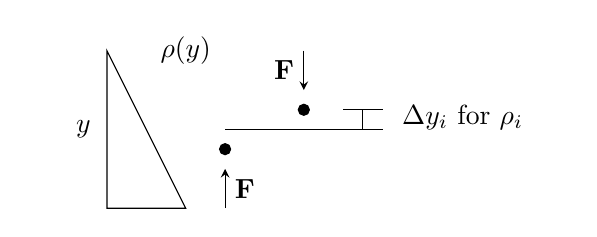
\begin{tikzpicture}
                \draw (0,0) -- (0,0);
                \draw (1,2) -- (1, 0) -- (2, 0) -- cycle;
                \node at (2.0, 2.0) {$\rho(y)$};
                \node at (0.7, 1) {$y$};

                \filldraw[black] (2.5,0.75) circle (2pt);
                \draw[-stealth] (2.5,0) --+ (0, .5);
                \node at (2.75, 0.25) {$\mathbf{F}$};

                \filldraw[black] (3.5,1.25) circle (2pt);
                \draw[-stealth] (3.5,2) --+ (0, -.5);
                \node at (3.25, 1.75) {$\mathbf{F}$};

                \draw (2.5,1) -- (4.5,1);
                \draw (4,1.25) -- (4.5,1.25);
                \draw (4.25,1.25) -- (4.25,1);
                \node[text width=2cm] at (5.75, 1.15) {$\Delta y_i$ for $\rho_i$}; 
            %   \draw[-stealth, ultra thick] (0,0) --+ (.6,.8);
            %   \draw[-stealth, ultra thick] (0,0) --+ (.3, -.6);
            \end{tikzpicture}
            \label{fig:strat_conv}
            \caption{Restoring force and equilibrium on particle $i$.}
        \end{figure}
        
        \begin{figure}
            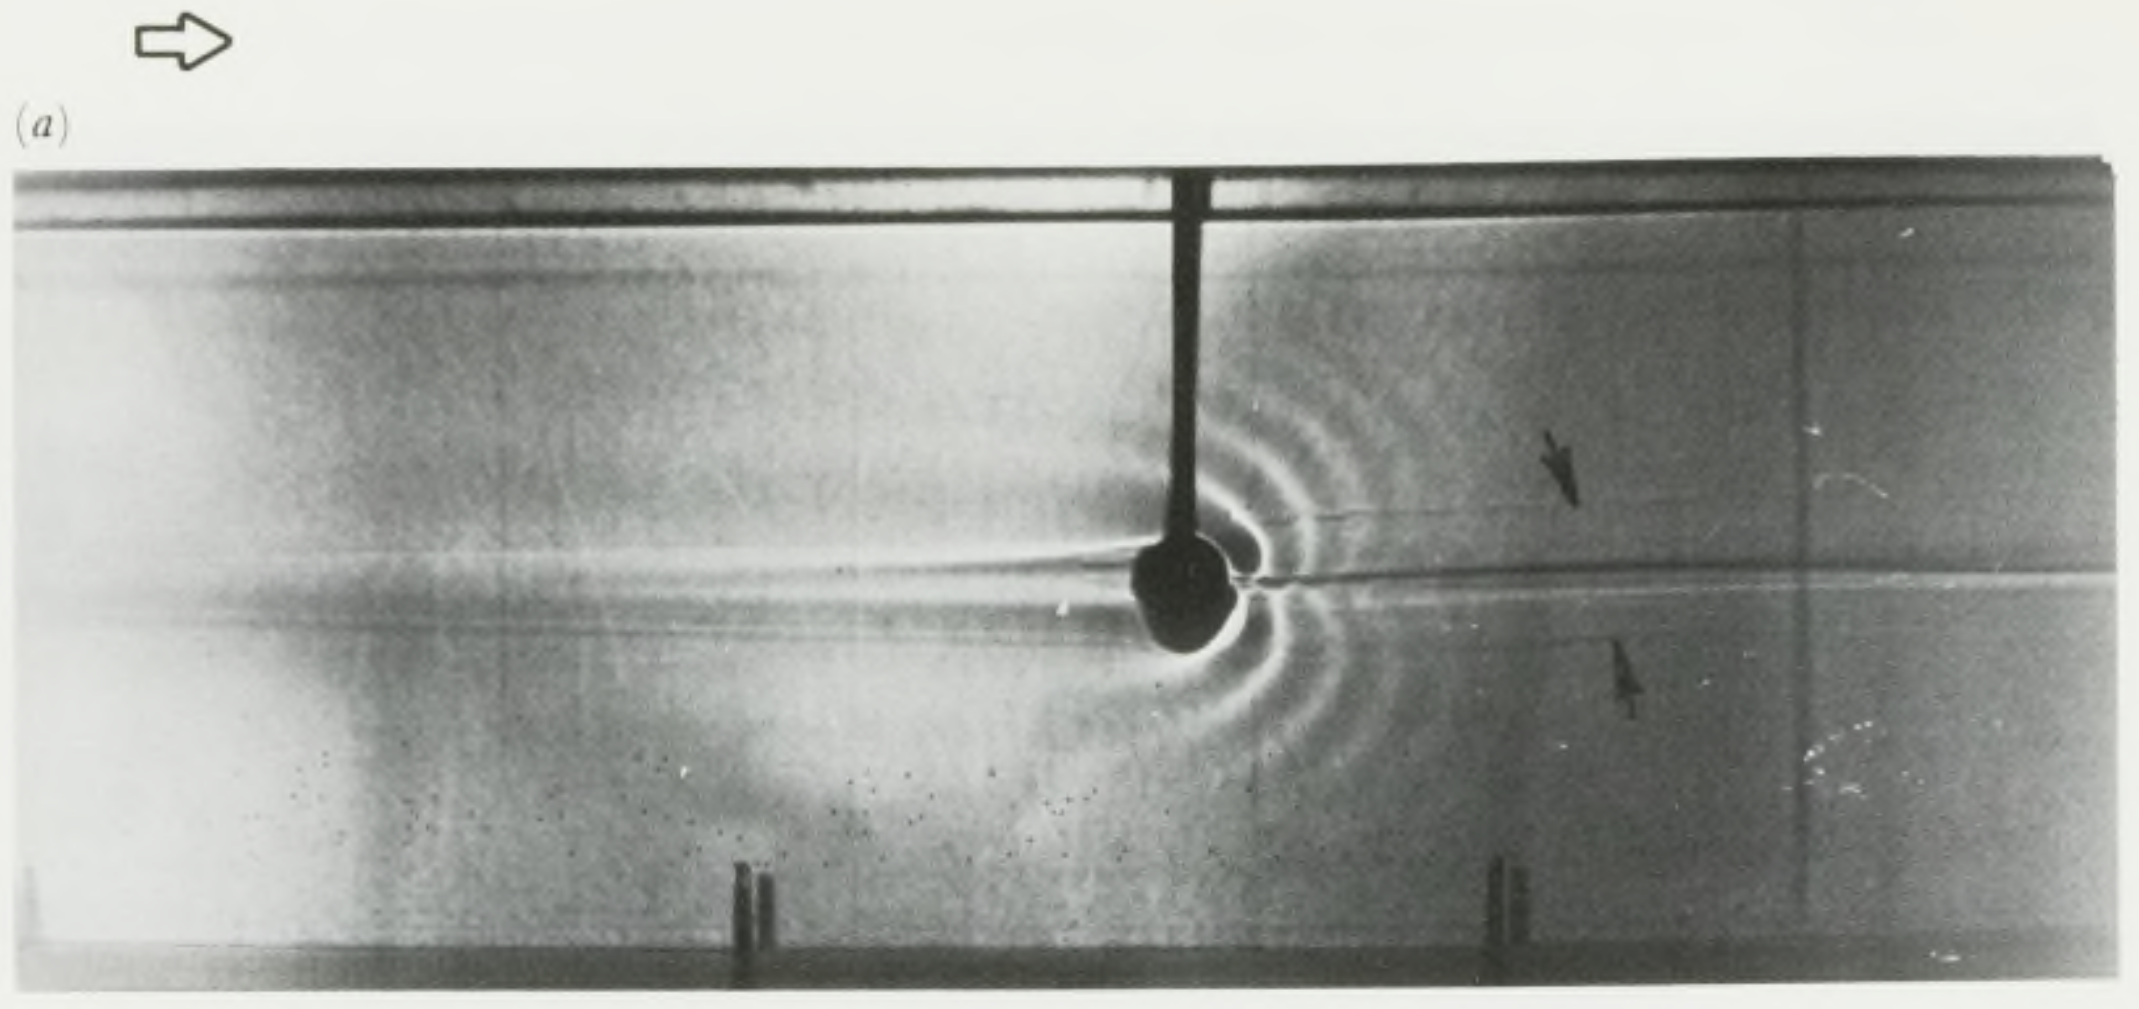
\includegraphics[width=.6\textwidth]{figures/boyer.png}
            \label{fig:boyer}
            \caption{Lee waves from flow past a cylinder \cite{boyer1989linearly}.}
        \end{figure}
        
        \column{.5\textwidth} % Left column and width
        %\textbf{Heading}
        \begin{itemize}
            \item In nature, there exist innumerable flows with varying density, known as stratified flows, such as the ocean.
            \item The density variation is caused by salt content or temperature variation.
            \item Stratified mediums exhibit a restoring force due to particles being in the lowest potential energy position when at the same depth as particles of similar density. 
            \item This force creates \textit{internal gravity waves}.
            \begin{itemize}
                \item Flow past a bluff body creates steady gravity waves known as \textit{lee waves}.
                \item Bluff body oscillation forms unsteady waves. 
            \end{itemize} 
        \end{itemize}
    \end{columns}
\end{frame}

%------------------------------------------------

\begin{frame}{Motivation}

    \begin{columns}[c]

        \column{.5\textwidth}    
        \begin{itemize}
            \item Internal gravity waves and other effects from stratfication affect the flow structures and forces on bodies. 
            \item Stratification is defined by the Densimetric Froude number.
            \begin{itemize}
                \item Lower Froude number means higher stratification.
            \end{itemize}
            \item Submersible bodies are approximated by slender bodies, and nonspherical bodies have been neglected in past studies. 
            \item \cite{ortiz2019stratified} look at static slender bodies; we introduce rotation.
            \item We want to better understand the dynamics of spheroidal bodies in stratified flows for design in submersible vehicles. 
        \end{itemize}

        \column{.5\textwidth}   
        \begin{figure}
            \centering
            \begin{subfigure}[b]{0.5\textwidth}
                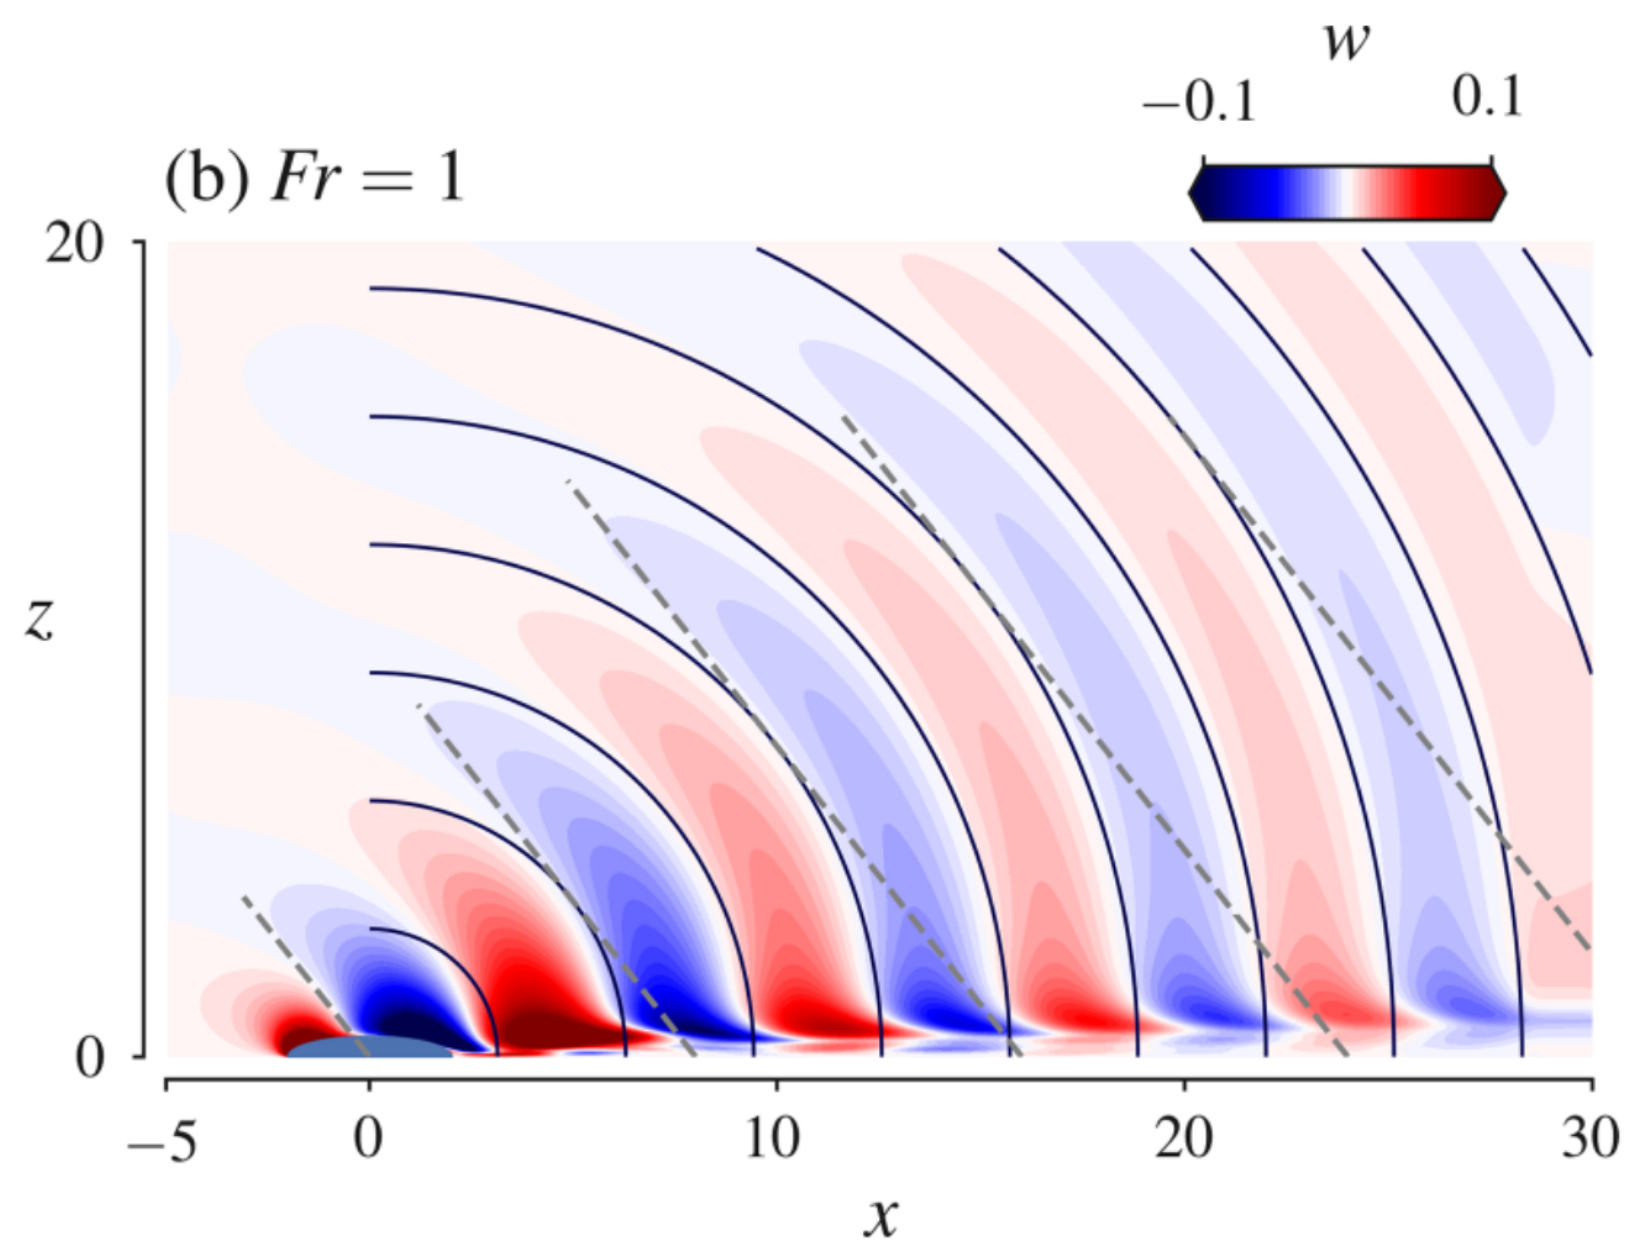
\includegraphics[width=\textwidth]{figures/bigviewIGW.png}
            \end{subfigure}\\
            \begin{subfigure}[b]{0.5\textwidth}
                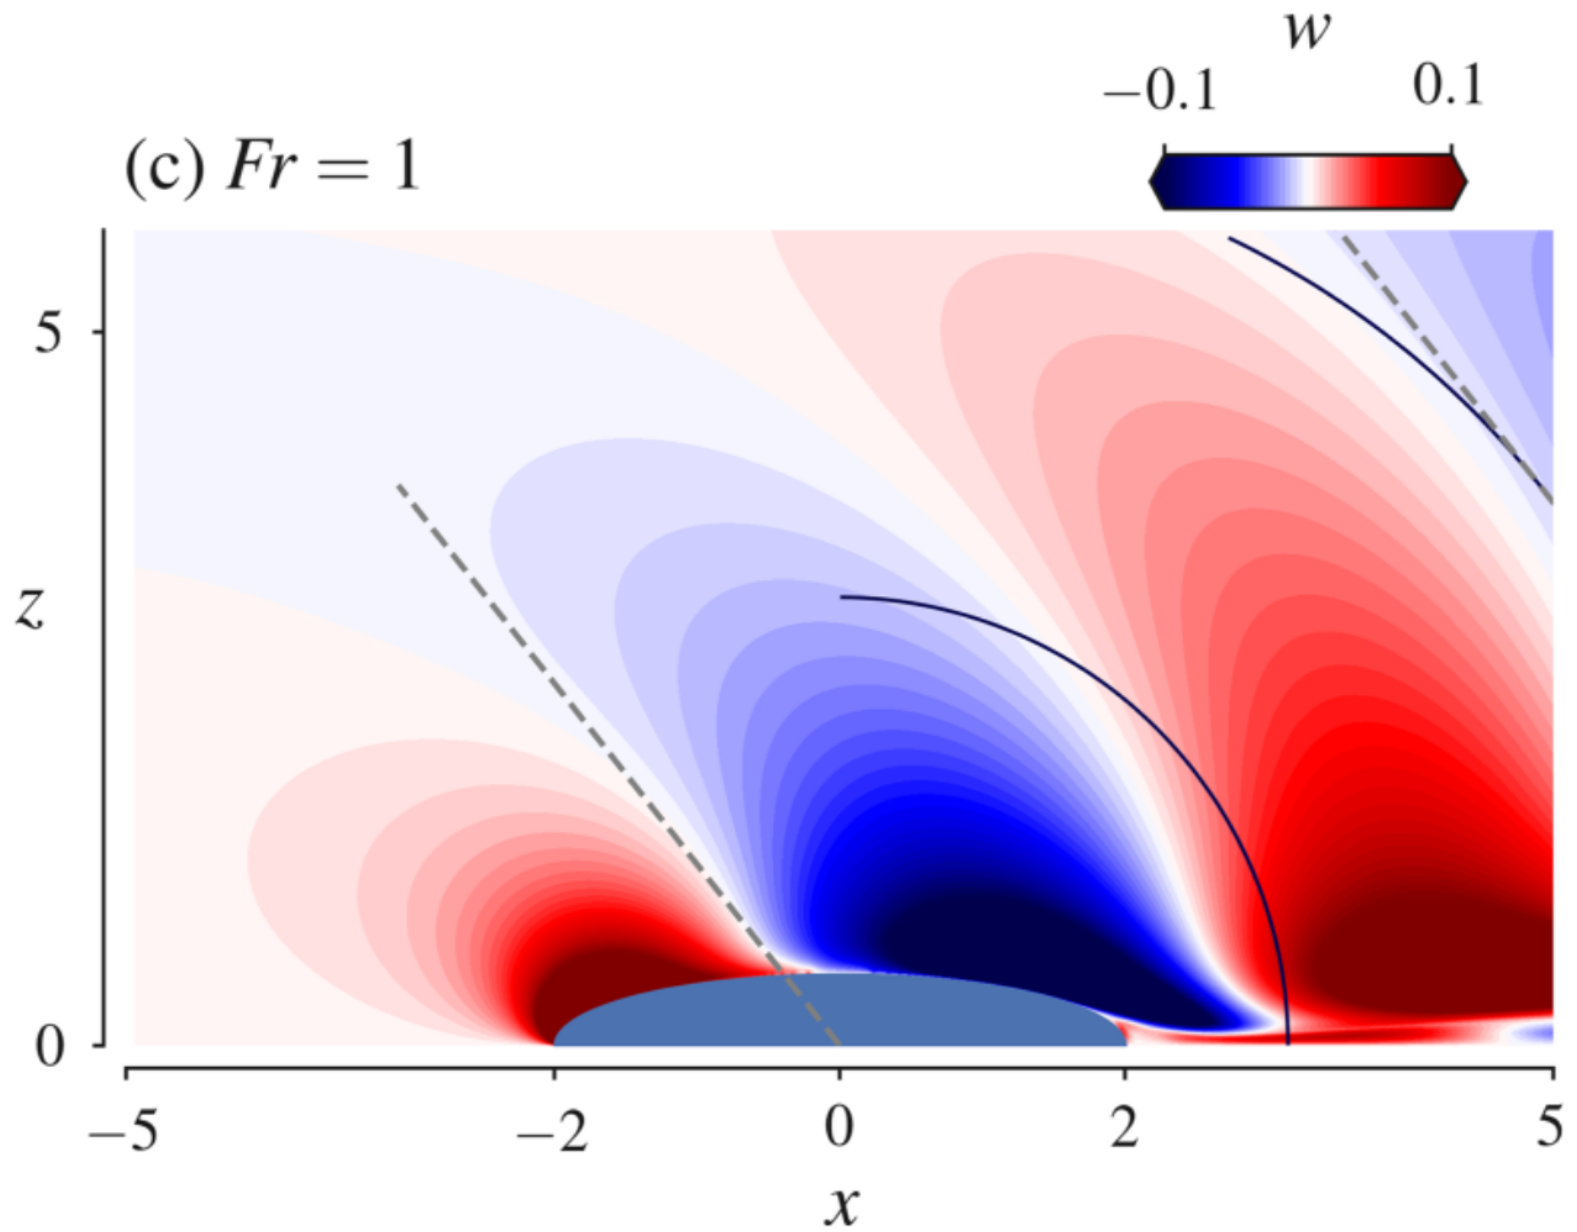
\includegraphics[width=\textwidth]{figures/smallviewIGW.png}
            \end{subfigure}
            \label{fig:ortiz}
            \caption{Internal gravity waves shown in the y-velocity fields \cite{ortiz2019stratified}.}
        \end{figure} 
%       \begin{itemize}
%       \end{itemize}
        
    \end{columns}
\end{frame}

%------------------------------------------------
\section{Methodology}
%------------------------------------------------

\begin{frame}{Equations and Setup}
    \small
    Incompressible Navier-Stokes Equations (\ref{eq:INSE}), with Boussinesq approximation and transport equation (\ref{eq:density transport}).
    
    \begin{equation}
        \label{eq:INSE}
        \frac{\partial\mathbf{u}}{\partial t}+\mathbf{u}\cdot\nabla\mathbf{u}=-\nabla p+\frac{1}{\Rey}\nabla^2\mathbf{u}-\frac{1}{{Fr}^2} (\rho^\prime\ -\ y )\hat{y}, \quad
        \nabla \cdot \textbf{u} = 0
    \end{equation}
    \begin{equation}
        \label{eq:density transport}
        \frac{\partial\rho '}{\partial t}+\mathbf{u}\cdot\nabla\rho'=\frac{1}{\Pran \Rey}\nabla^2\rho '
    \end{equation}   
    \vspace{-5pt} 
    \begin{columns}[c]
        \column{.5\textwidth}
        \begin{figure}
            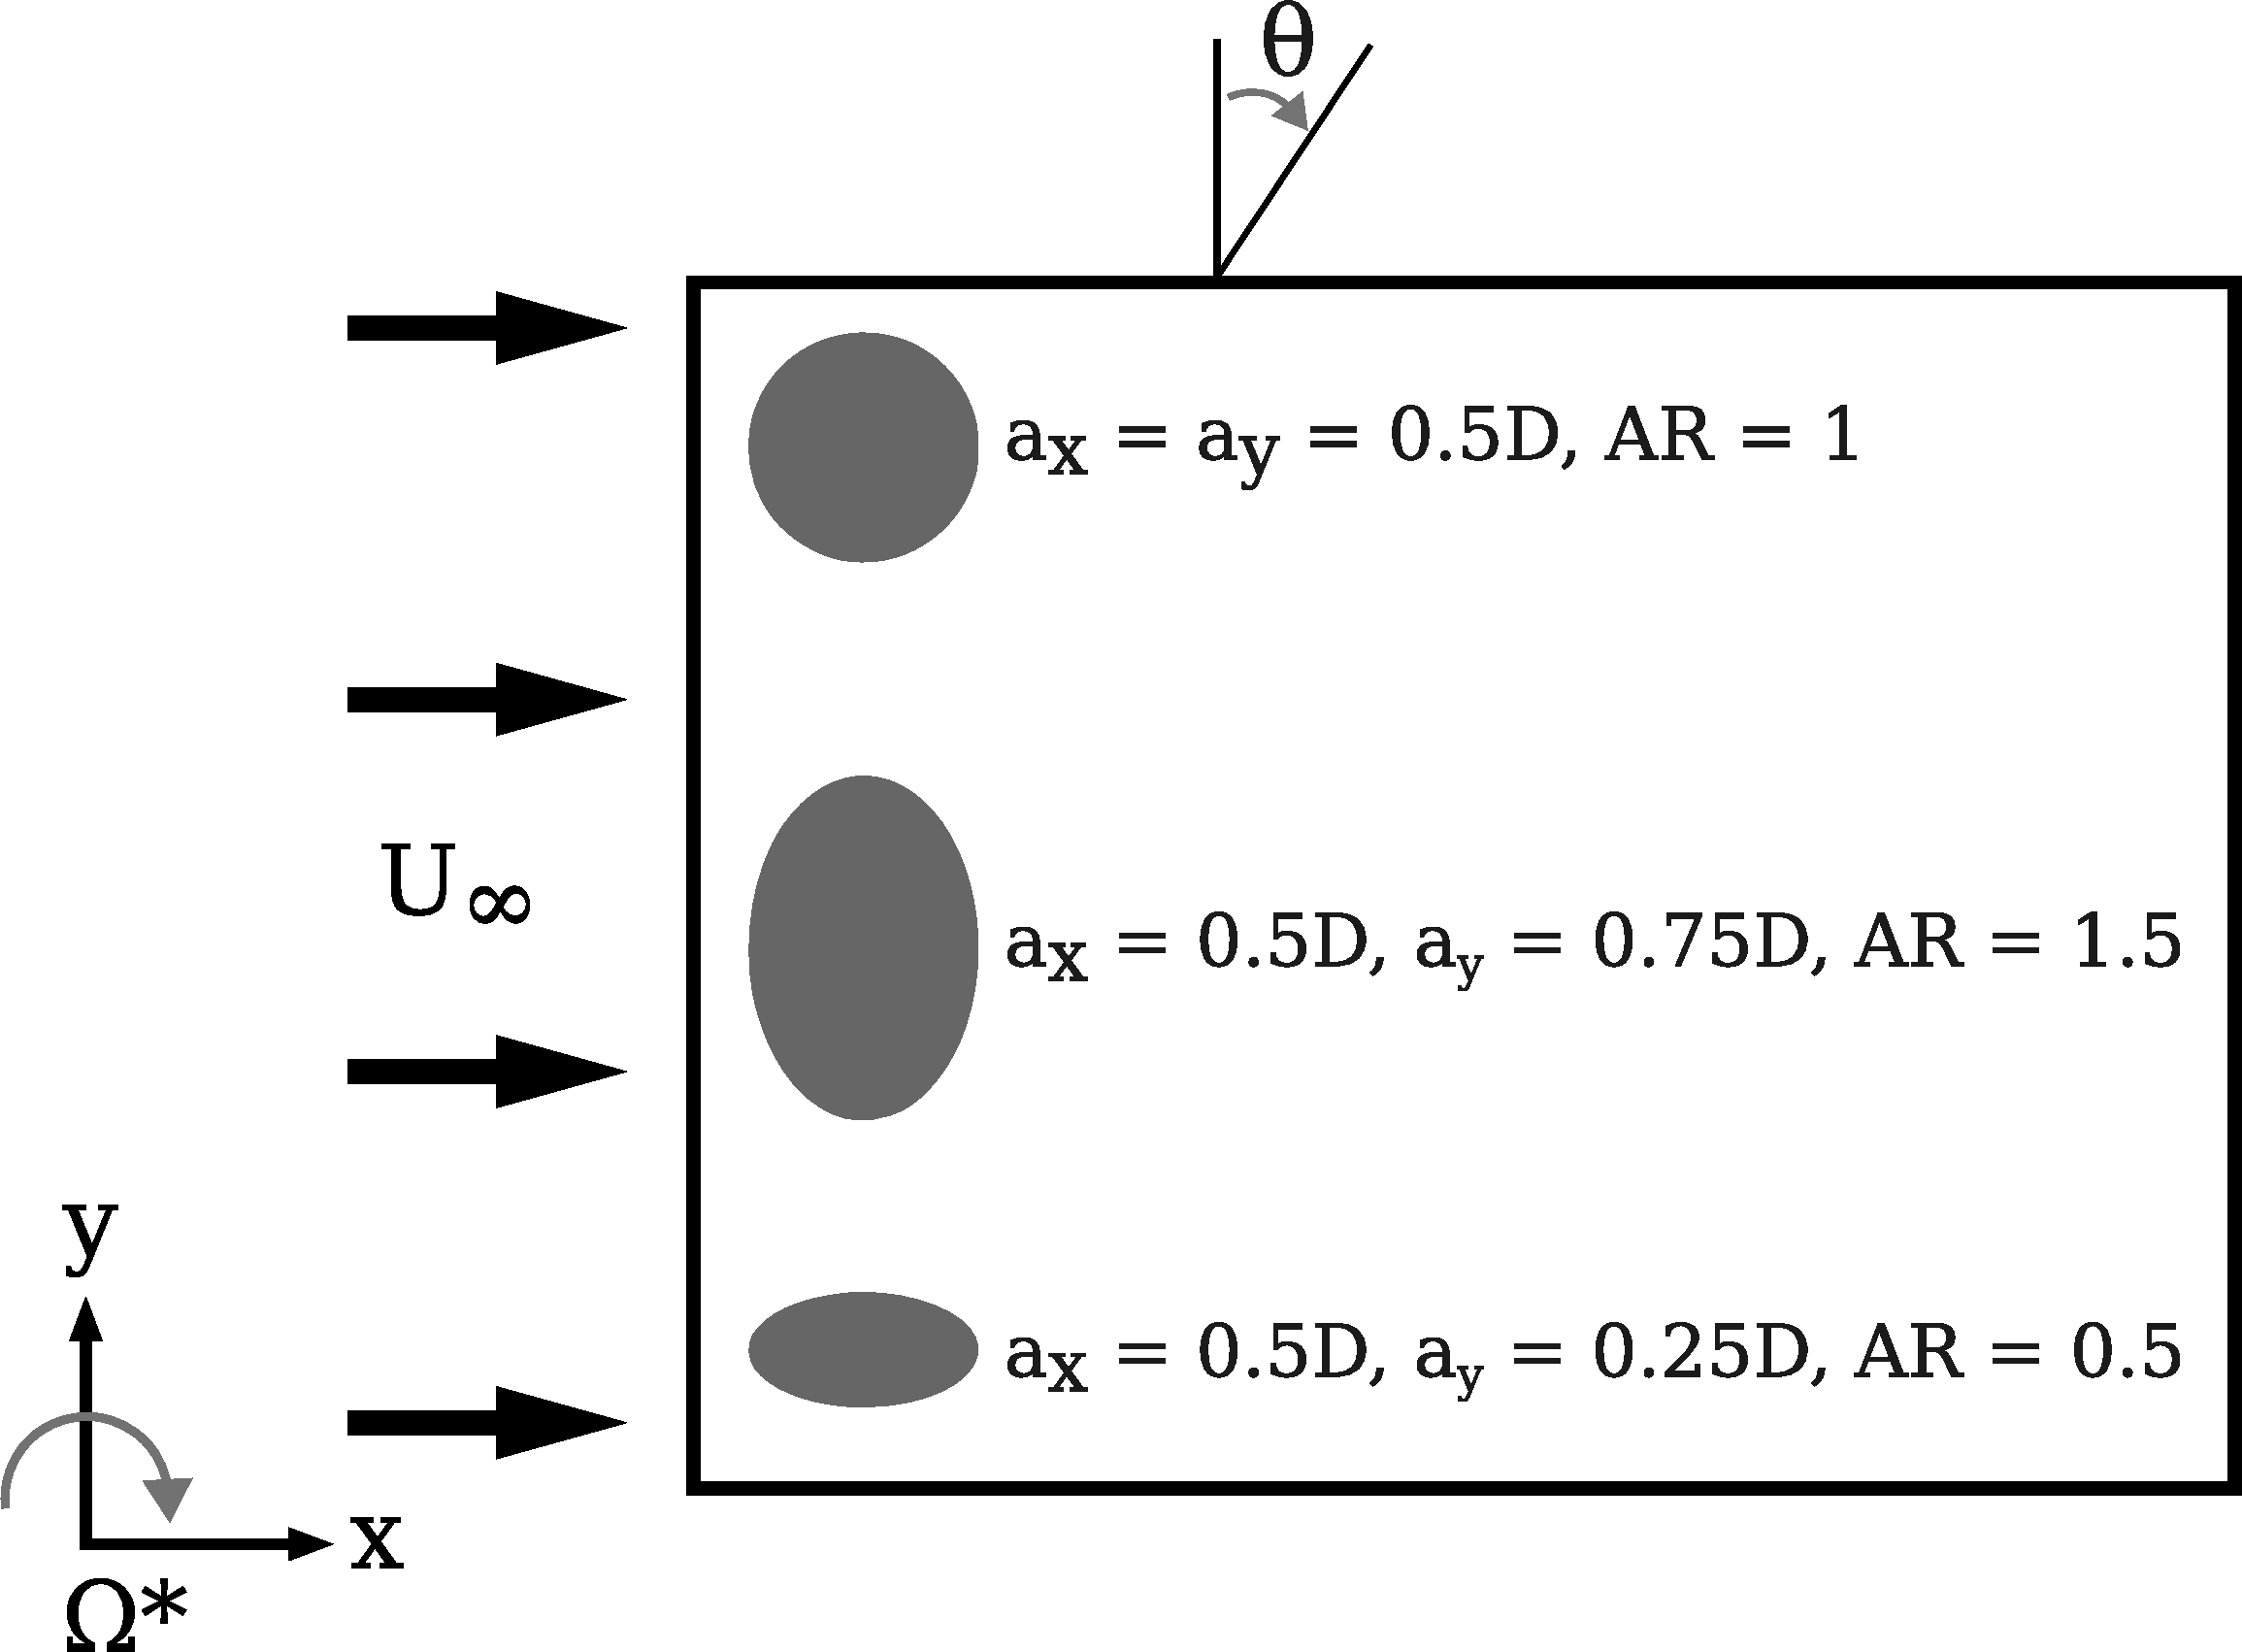
\includegraphics[width=.8\textwidth]{figures/flow_setup.pdf}
        \end{figure}
        \column{.5\textwidth}
        \begin{itemize}
            \item Density perturbation $\rho^{\prime}$ from background density $\rho_0$.
            \item Thermal diffusivity $\kappa$, kinematic viscosity $\nu$
            \item Aspect ratio $AR = a_y / a_x$, with $\Omega^{\ast} = \frac{\Omega D}{2 U_{\infty}}$
            \item Brunt–Väisälä frequency $N_{BV} = \bigg( \frac{g}{\rho_0} \rho^{\prime}_{y,0} \bigg)^{1/2}$
        \end{itemize}
        \[\Rey = \rho_0 \frac{U D}{\mu}, \Pran = \rho_0 \frac{\kappa}{\mu}, Fr^{-2}=\frac{gD^2}{\rho_0 U^2}|\rho^{\prime}_{y,0}|\]
    \end{columns}
    \normalsize
\end{frame}

%------------------------------------------------

\begin{frame}{Numerical Methodology - Temporal Discretization}
    \begin{columns}[c]
        \column{.5\textwidth}
        \begin{itemize}
            \item Semi-implicit BDF-3/EXT-3 timestepping
            \begin{itemize}
                \item Time derivative - BDF-3
                \item Nonlinear terms - EXT-3
                \item Pressure and viscous terms - implicit
            \end{itemize}
            \item Spatially interpolated boundary conditions at interdomain boundaries \cite[]{mittal2019nonconforming}.
            \begin{itemize}
                \item Picard iterations
                \item M-order temporal extrapolation at boundaries for accuracy
                \item Q corrector iterations for stability
            \end{itemize}
            \item Arbitrary Lagrangian-Eulerian (ALE) formulation to track spinning inner mesh.
            \item Method allows better shape adaptation.
            \item Spectral accuracy retained
        \end{itemize}
        \column{.5\textwidth}
        \begin{figure}
            \animategraphics[loop,autoplay,controls,width=.4\linewidth]{25}{spin_mesh/spin_mesh.}{0}{100}
        \end{figure}
    \end{columns}
\end{frame}

%------------------------------------------------

\begin{frame}{Numerical Methodology - Spatial Discretization}
    \begin{columns}[c]
        \column{.5\textwidth}
        \begin{itemize}
            \item Spectrally accurate overset grid method 
            \begin{itemize} 
                \item Inner mesh ($\Omega^{1}: 512$ elements)
                \item Outer mesh ($\Omega^{2}: 3200$ elements)
            \end{itemize}
            \item Schwarz-Spectral Element Method (Schwarz-SEM)
            \item Hexahedral elements
            \item Symmetric top and bottomr boundaries
            \item Lagrangle polynomials
            
            
        \end{itemize}
      
        \begin{table}
            \centering
            \begin{tabular}{c|c}
              Parameters      & Values   \\ \hline
              $AR$   & $0.5, 1.0, 1.5$ \\
              $Fr^2$ & $0.01, 0.1, 1.0, 10.0, 100.0, \infty$     \\
              $\Rey$ & $120$  \\
              $\Pr$ & $1$  \\
              $\Omega^{\ast}$ & $0.0$ ($AR = 1$ only), $1.0$  \\
            \end{tabular}
            \label{table:parameter_space}
        \end{table}
        
        \column{.5\textwidth}
        \begin{itemize}
            \item Polynomial order $N = 11$
            \item Gauss-Lobatto-Legendre (GLL) nodes
        \end{itemize}
        \begin{figure}
            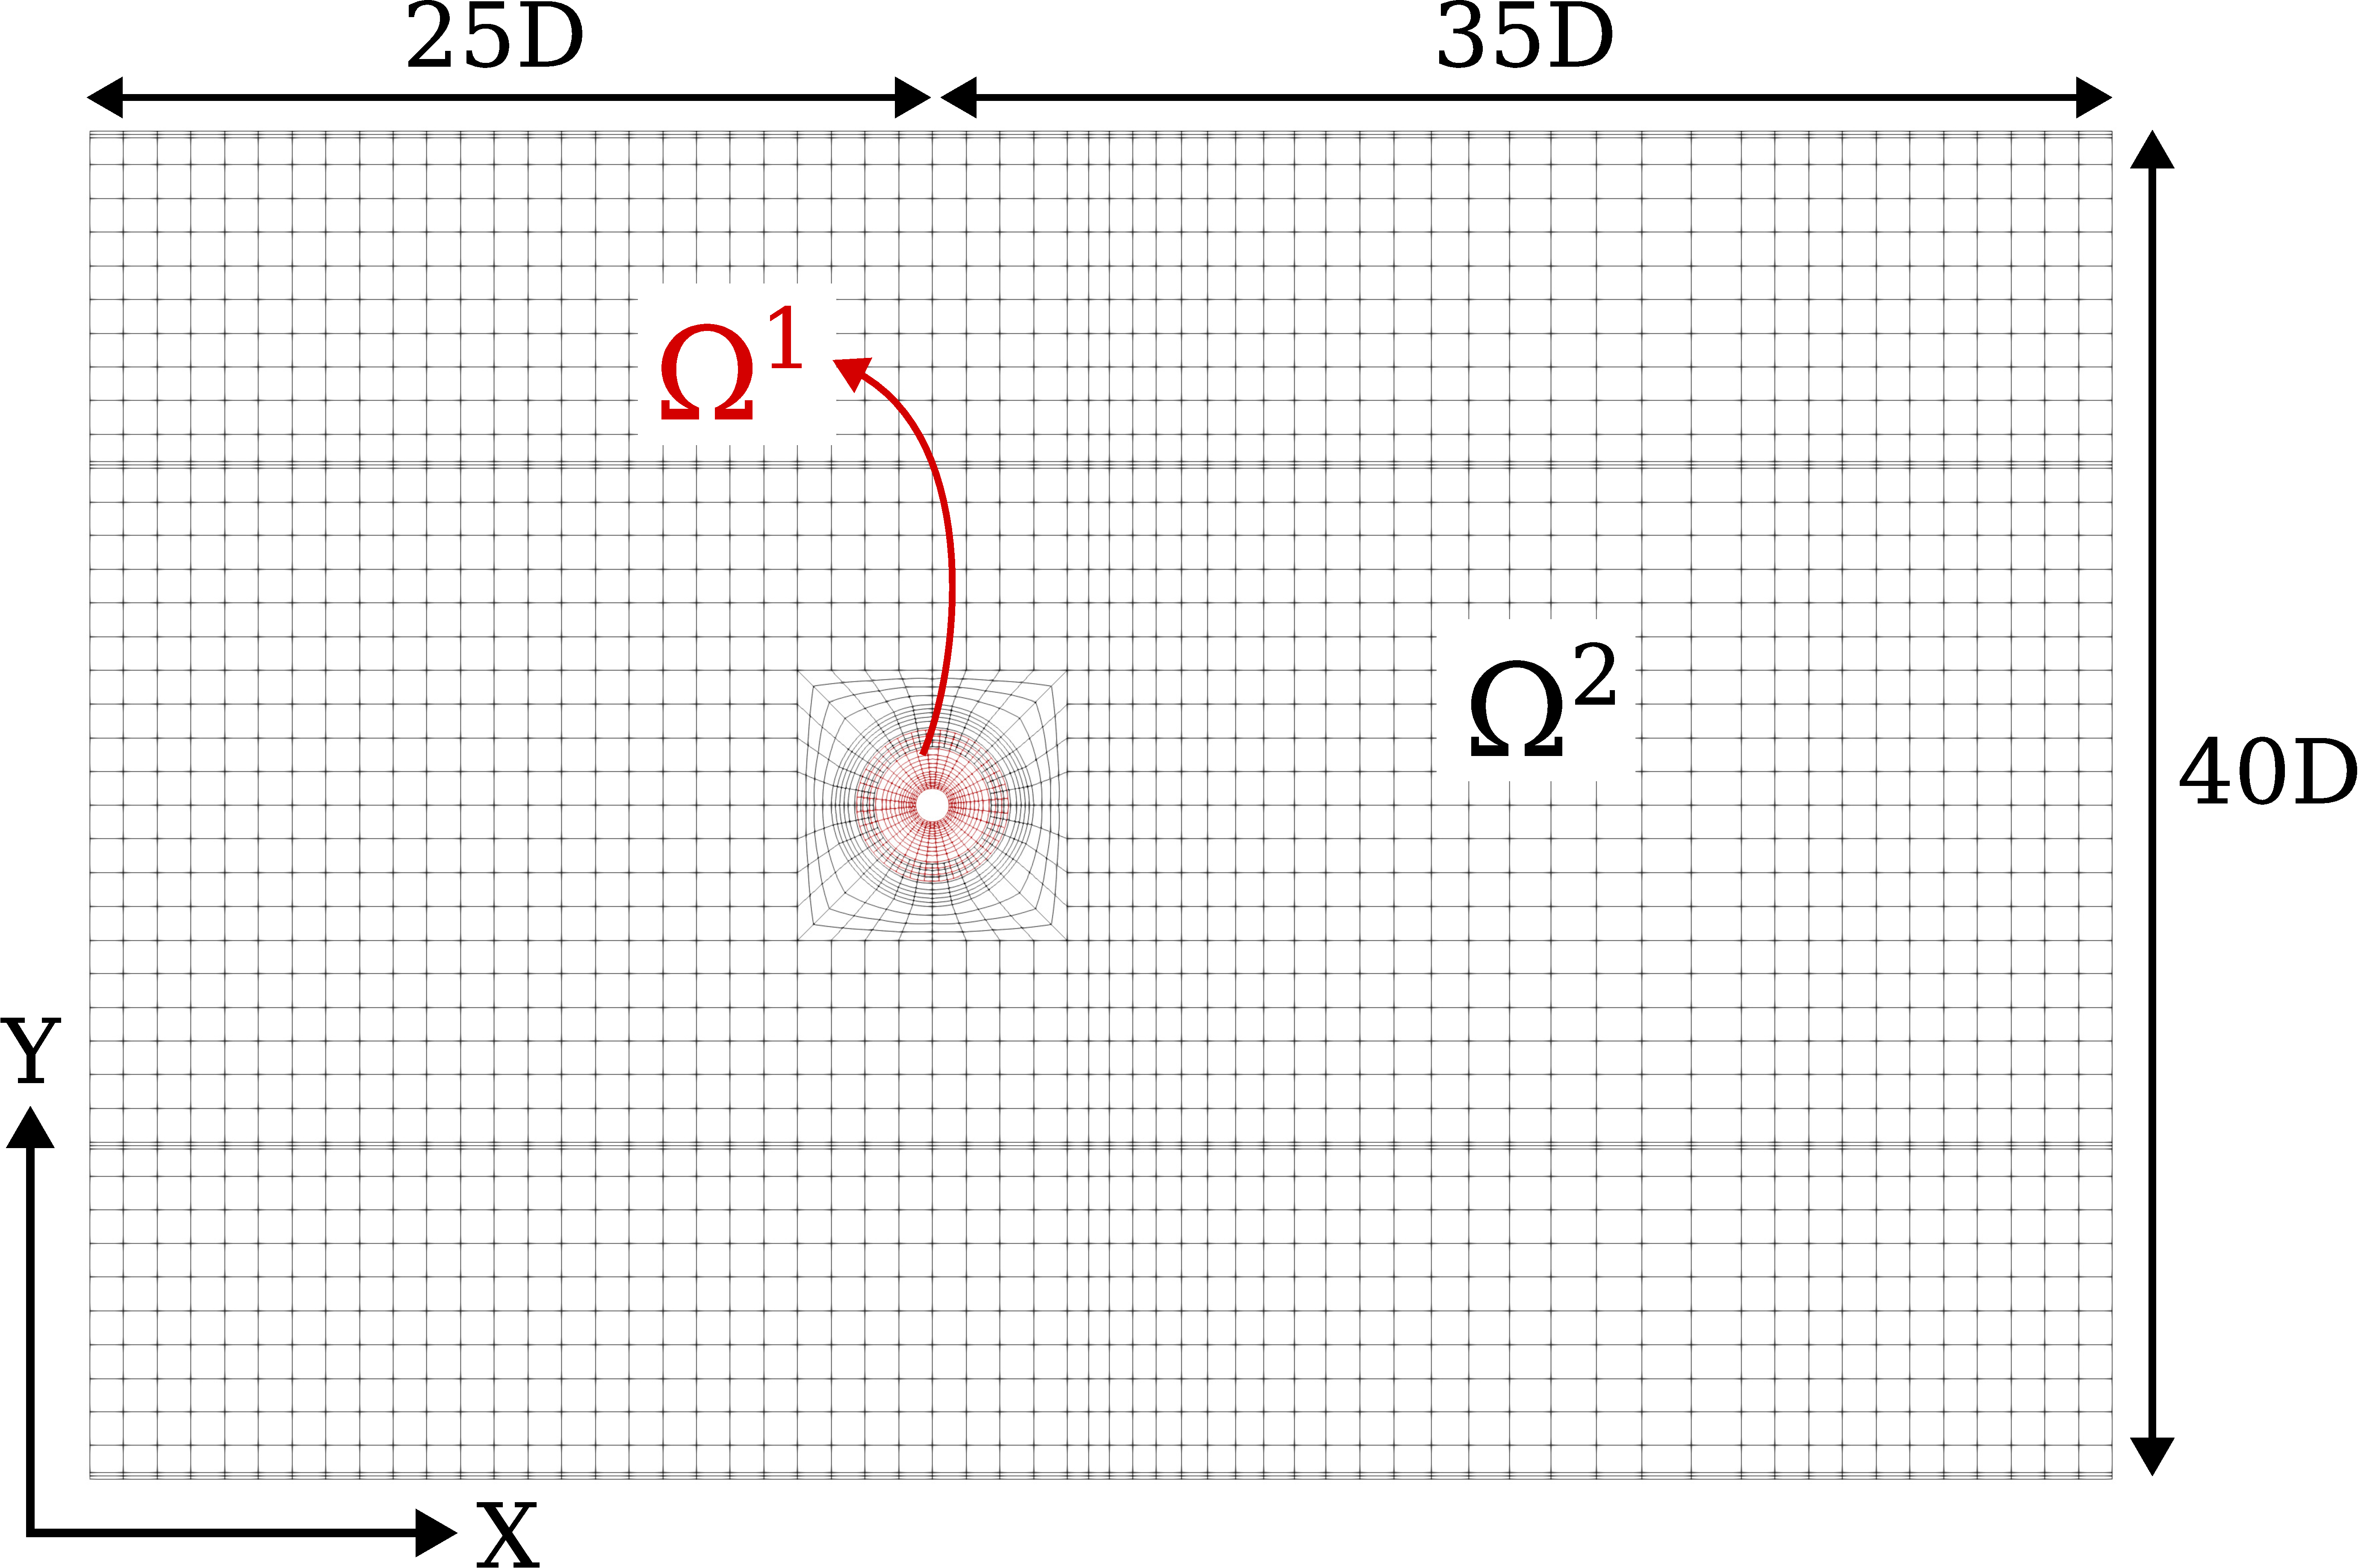
\includegraphics[width=\textwidth]{figures/mesh.pdf}
        \end{figure}
            \footnotesize
            \textsuperscript{1}https://nek5000.mcs.anl.gov/
            \normalsize 
    \end{columns}
\end{frame}

%------------------------------------------------

\begin{frame}{Validation}
    We validate Schwarz-SEM stratification implementation in two ways.
    First, by validating nonrotating stratified cases against monodomain stratified cases. 
    Second, by comparing rotating unstratified cases with rotating unstratified cases from \cite{lu2018flow} (two papers) produced with \textit{Ansys\textsuperscript{\textregistered} Fluent} with \textit{Sliding Mesh}. 
    Drag and lift show similarity.  
    \begin{columns}[c]
        \column{.3\textwidth}
        \begin{figure}
            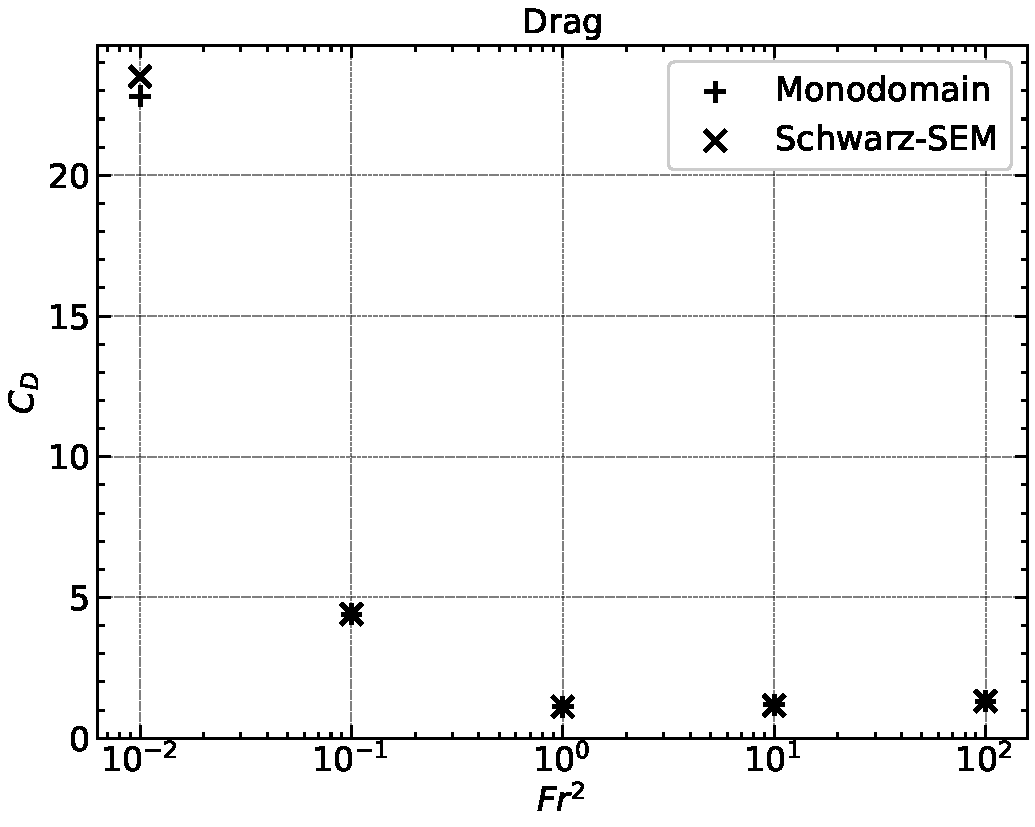
\includegraphics[width=\textwidth]{figures/dragvalnn.pdf}
            \caption{Comparision of drag against monodomain case.}
        \end{figure}
        \column{.7\textwidth}
        \begin{figure}
            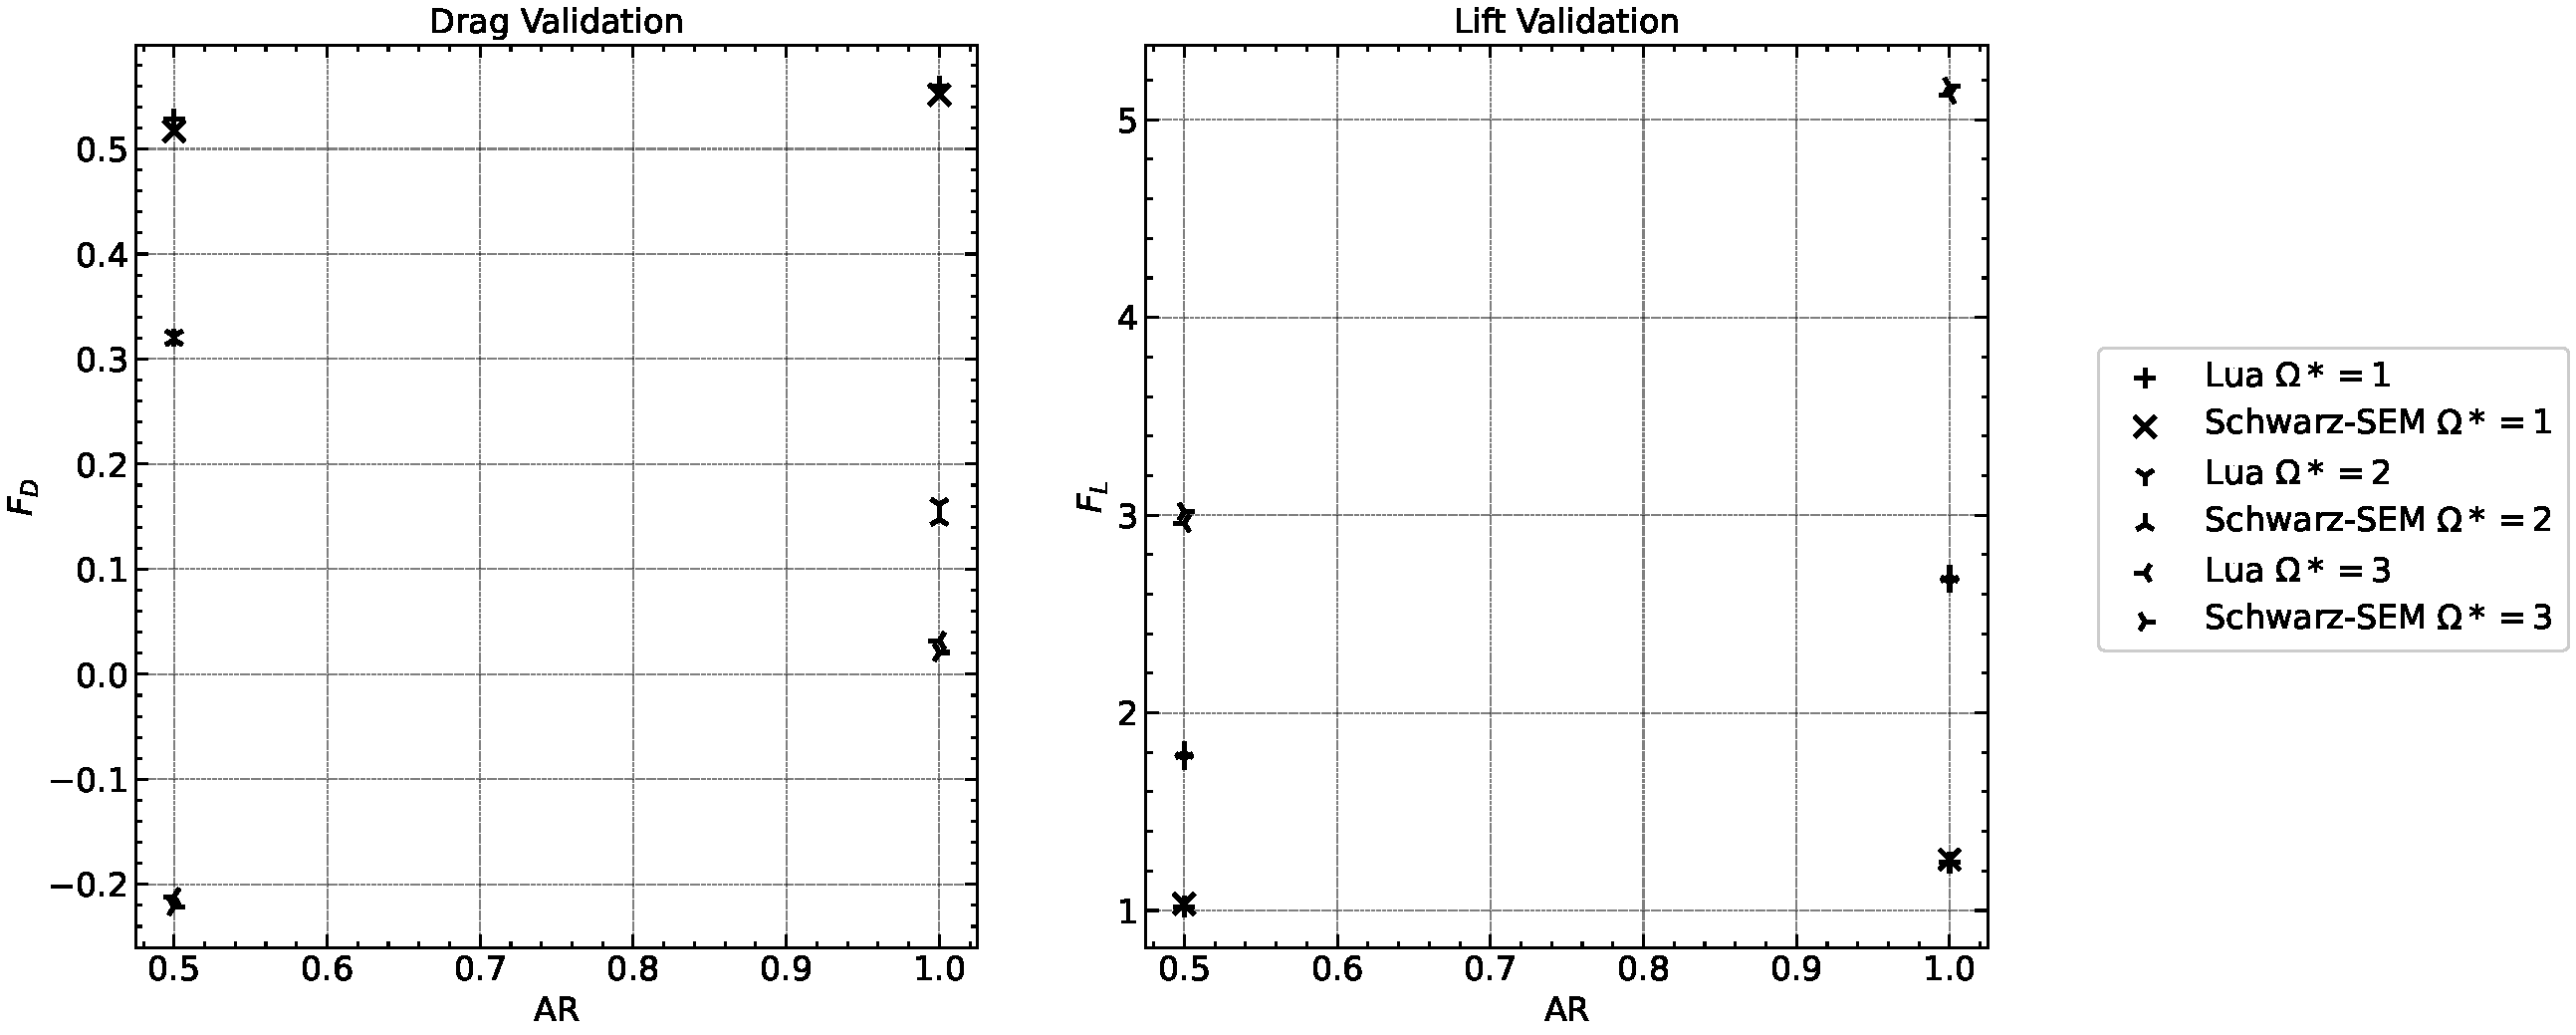
\includegraphics[width=\textwidth]{figures/lua_com.pdf}
            \caption{Comparison of drag and lift in unstratified flow against \cite{lu2018flow} finite-volume results at $\Rey = 200$}.
        \end{figure}
    \end{columns}
    
\end{frame}

%------------------------------------------------

\begin{frame}{Circle Drag and Lift Time Series}
    \begin{columns}[c]
        \column{.6\textwidth}
        \begin{figure}
            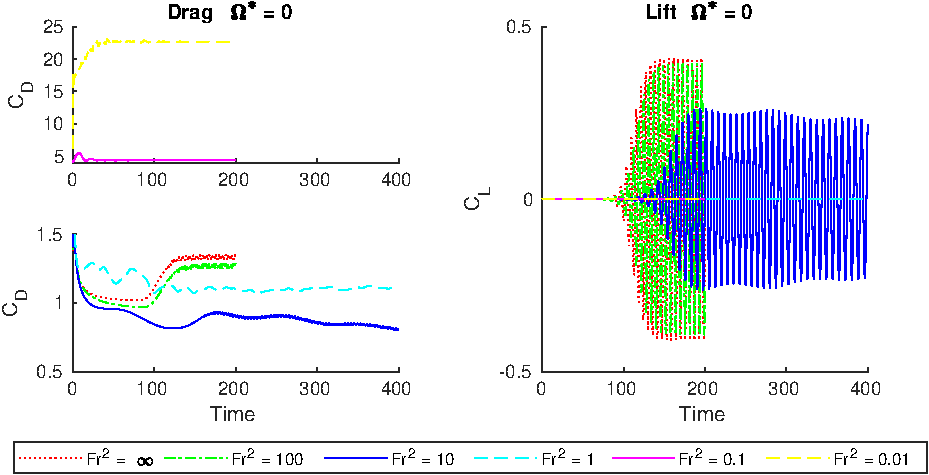
\includegraphics[width=.7\textwidth]{figures/timens.pdf}
        \end{figure}
        \begin{figure}
            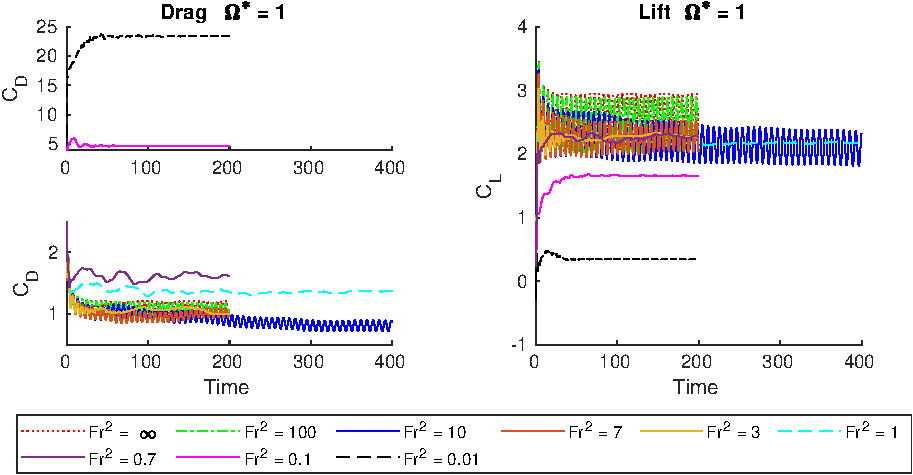
\includegraphics[width=.7\textwidth]{figures/times.pdf}
        \end{figure}
        \column{.4\textwidth}
        \begin{itemize}
            \item The plots to the left show time series data for nonspinning and spinning cyclinders.
            \item We observe the presence of different flow regimes
            \begin{itemize}
                \item A regime in which stratification dominates and there is little oscillation in lift
                \item A regime in which vortex-shedding dominates and there is substantial oscillation in lift.
            \end{itemize}
            \item The increase in drag with stratification increase if a result of upstream blocking.  
        \end{itemize}
    \end{columns}
\end{frame}

%------------------------------------------------

\begin{frame}{Circle Drag and Lift}
    \begin{columns}[c]
        \column{.70\textwidth}
        \begin{figure}
            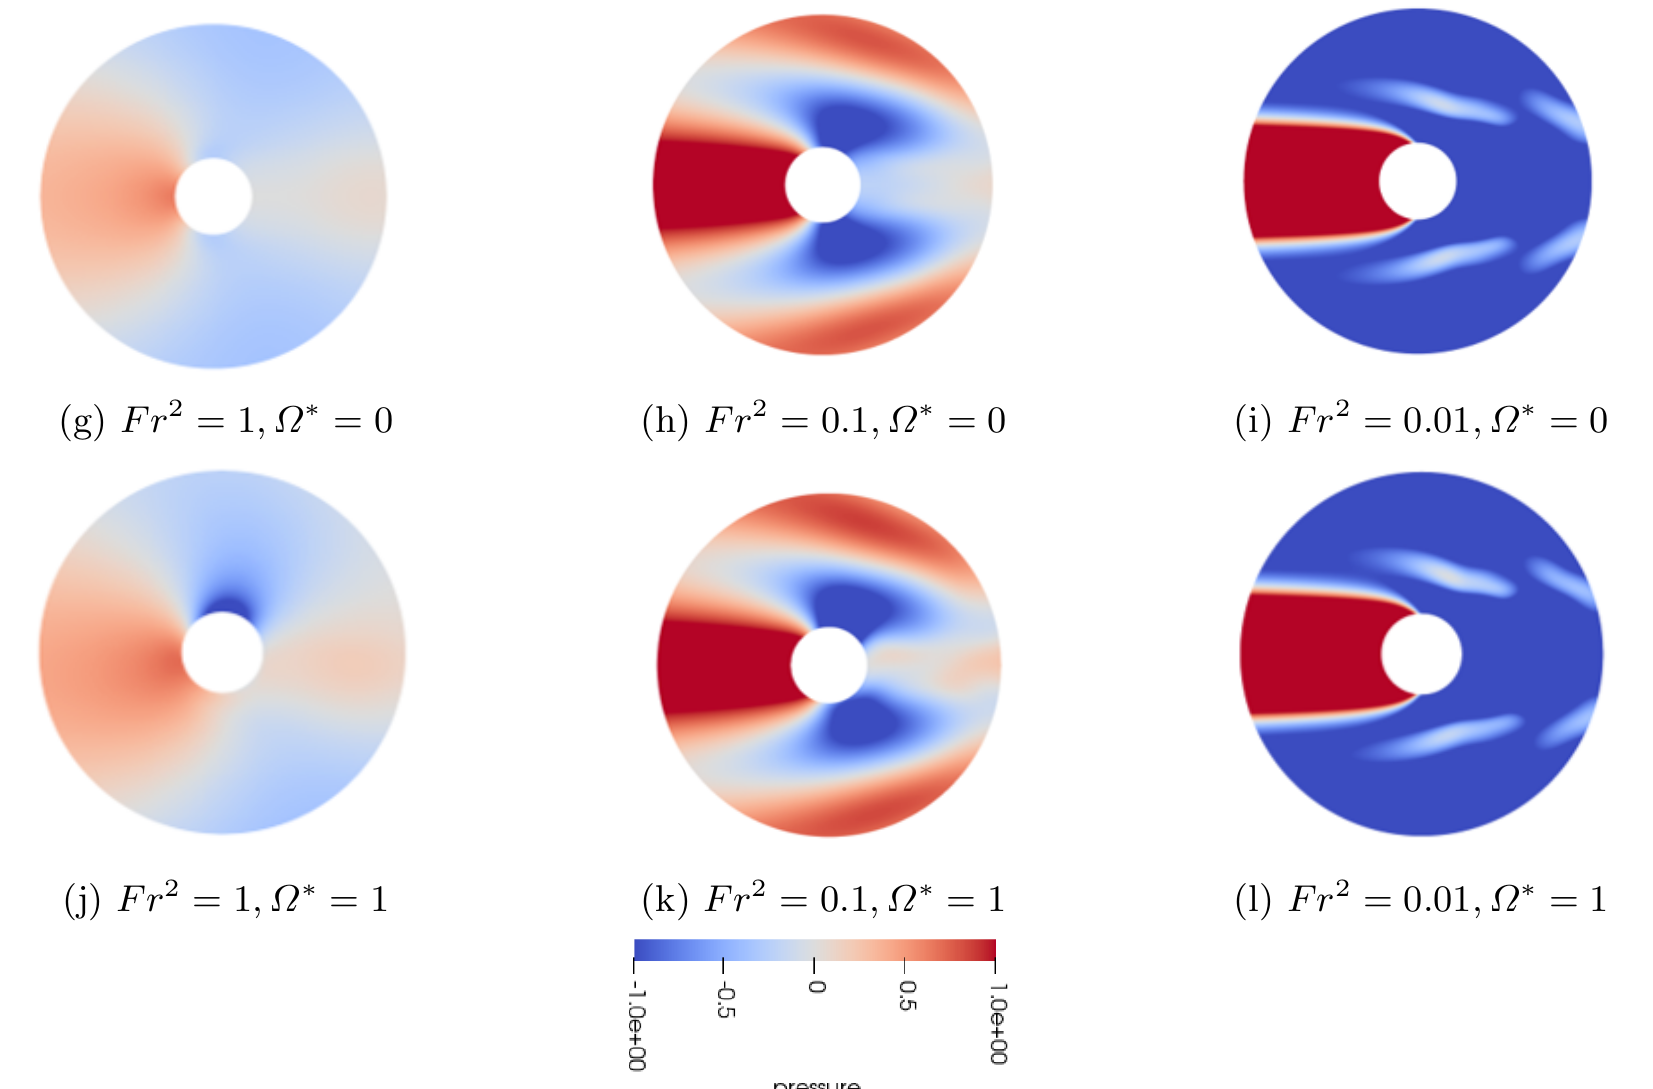
\includegraphics[width=.9\textwidth]{figures/circlepressure.png}
            \caption{Pressure distribution around 2D cylinders. High pressure region in front of the body at high stratification is upstream blocking.}
        \end{figure}
        \column{.20\textwidth}
        \vspace{-5pt}
        \begin{figure}
            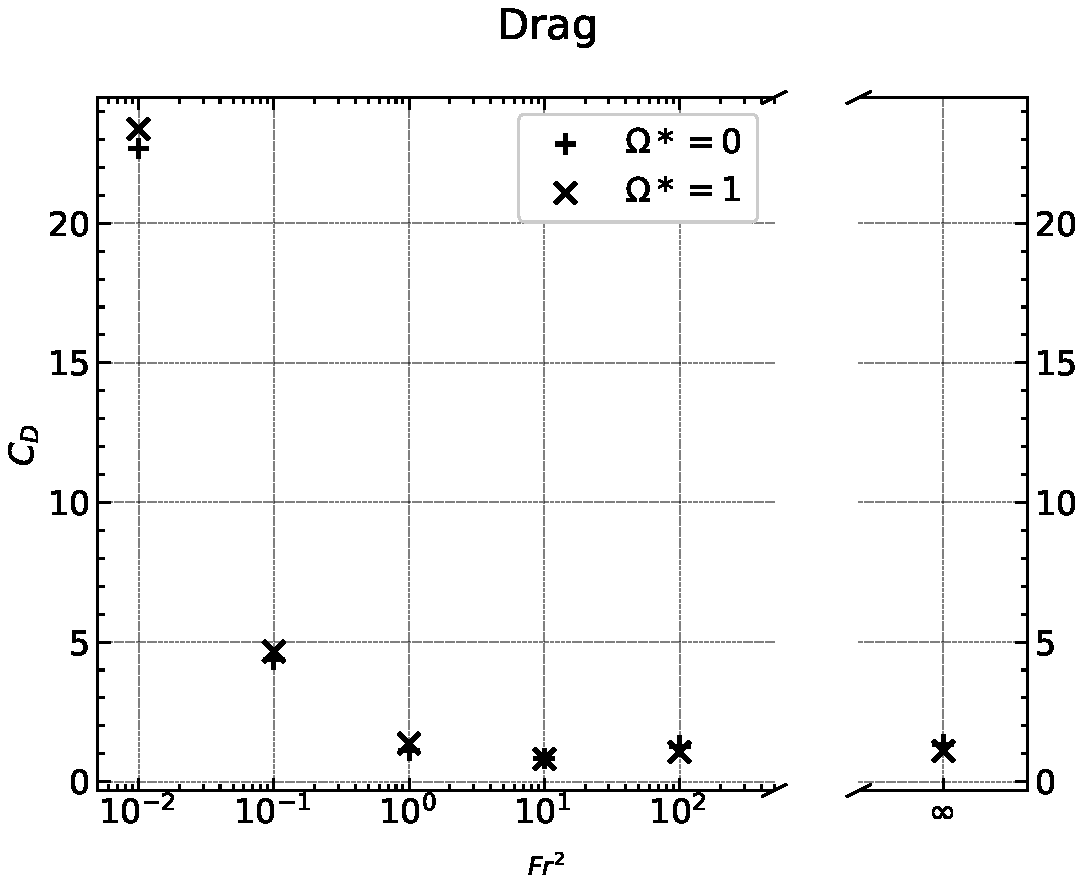
\includegraphics[width=\textwidth]{figures/circledrag.pdf}
            \caption{Mean Drag Coefficients}
        \end{figure}
        \vspace{-10pt}
        \begin{figure}
            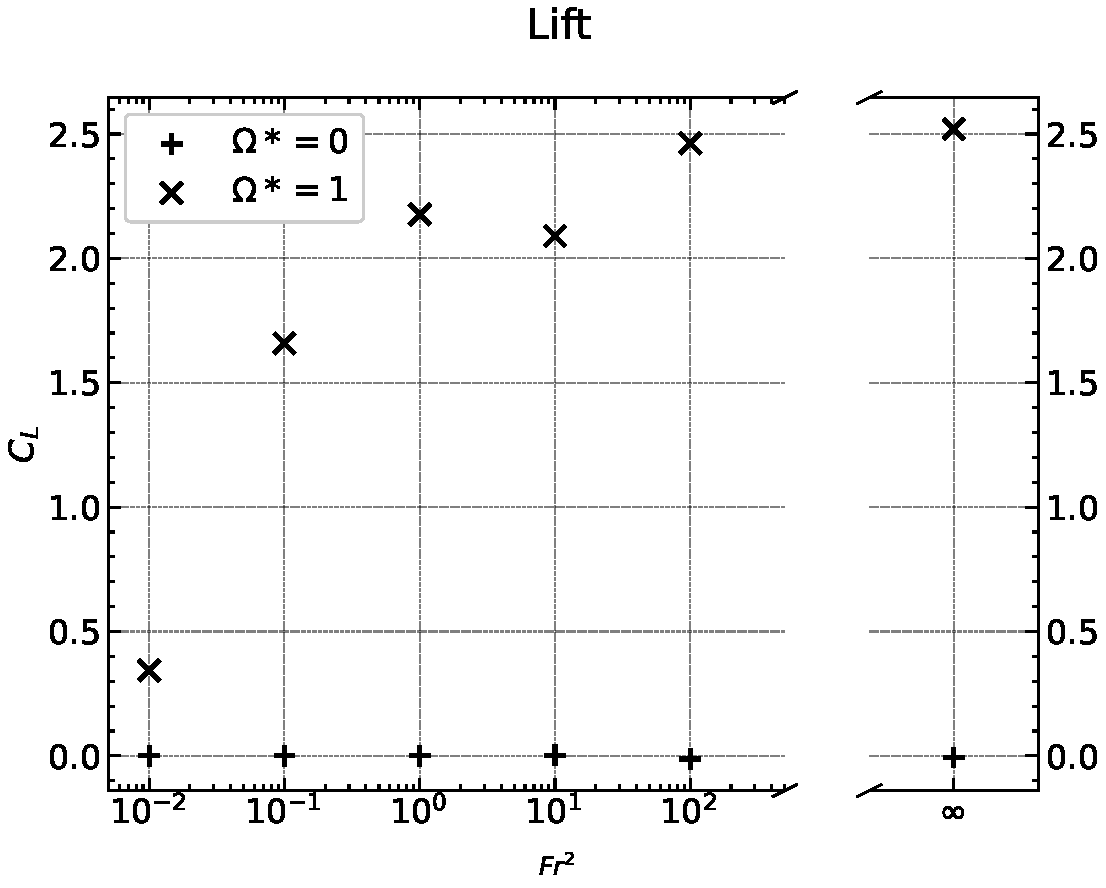
\includegraphics[width=\textwidth]{figures/circlelift.pdf}
            \caption{Mean Lift Coefficients}
        \end{figure}
    \end{columns}
\end{frame}

%------------------------------------------------

\begin{frame}{Circle Schlieren Plots}
    \begin{columns}[c]
        \column{.4\textwidth}
        \begin{itemize}
            \item The following plots are Schlieren plots calculated with density gradient $|\nabla \rho|$ 
            \item We observe the presence of different flow regimes
            \begin{itemize}
                \item A regime in which stratification dominates
                \item A regime in which vortex-shedding dominates
            \end{itemize}
            \item There exists a transitional regime at $Fr^2 \approx 10$
        \end{itemize}
        \column{.6\textwidth}
        \begin{figure}
            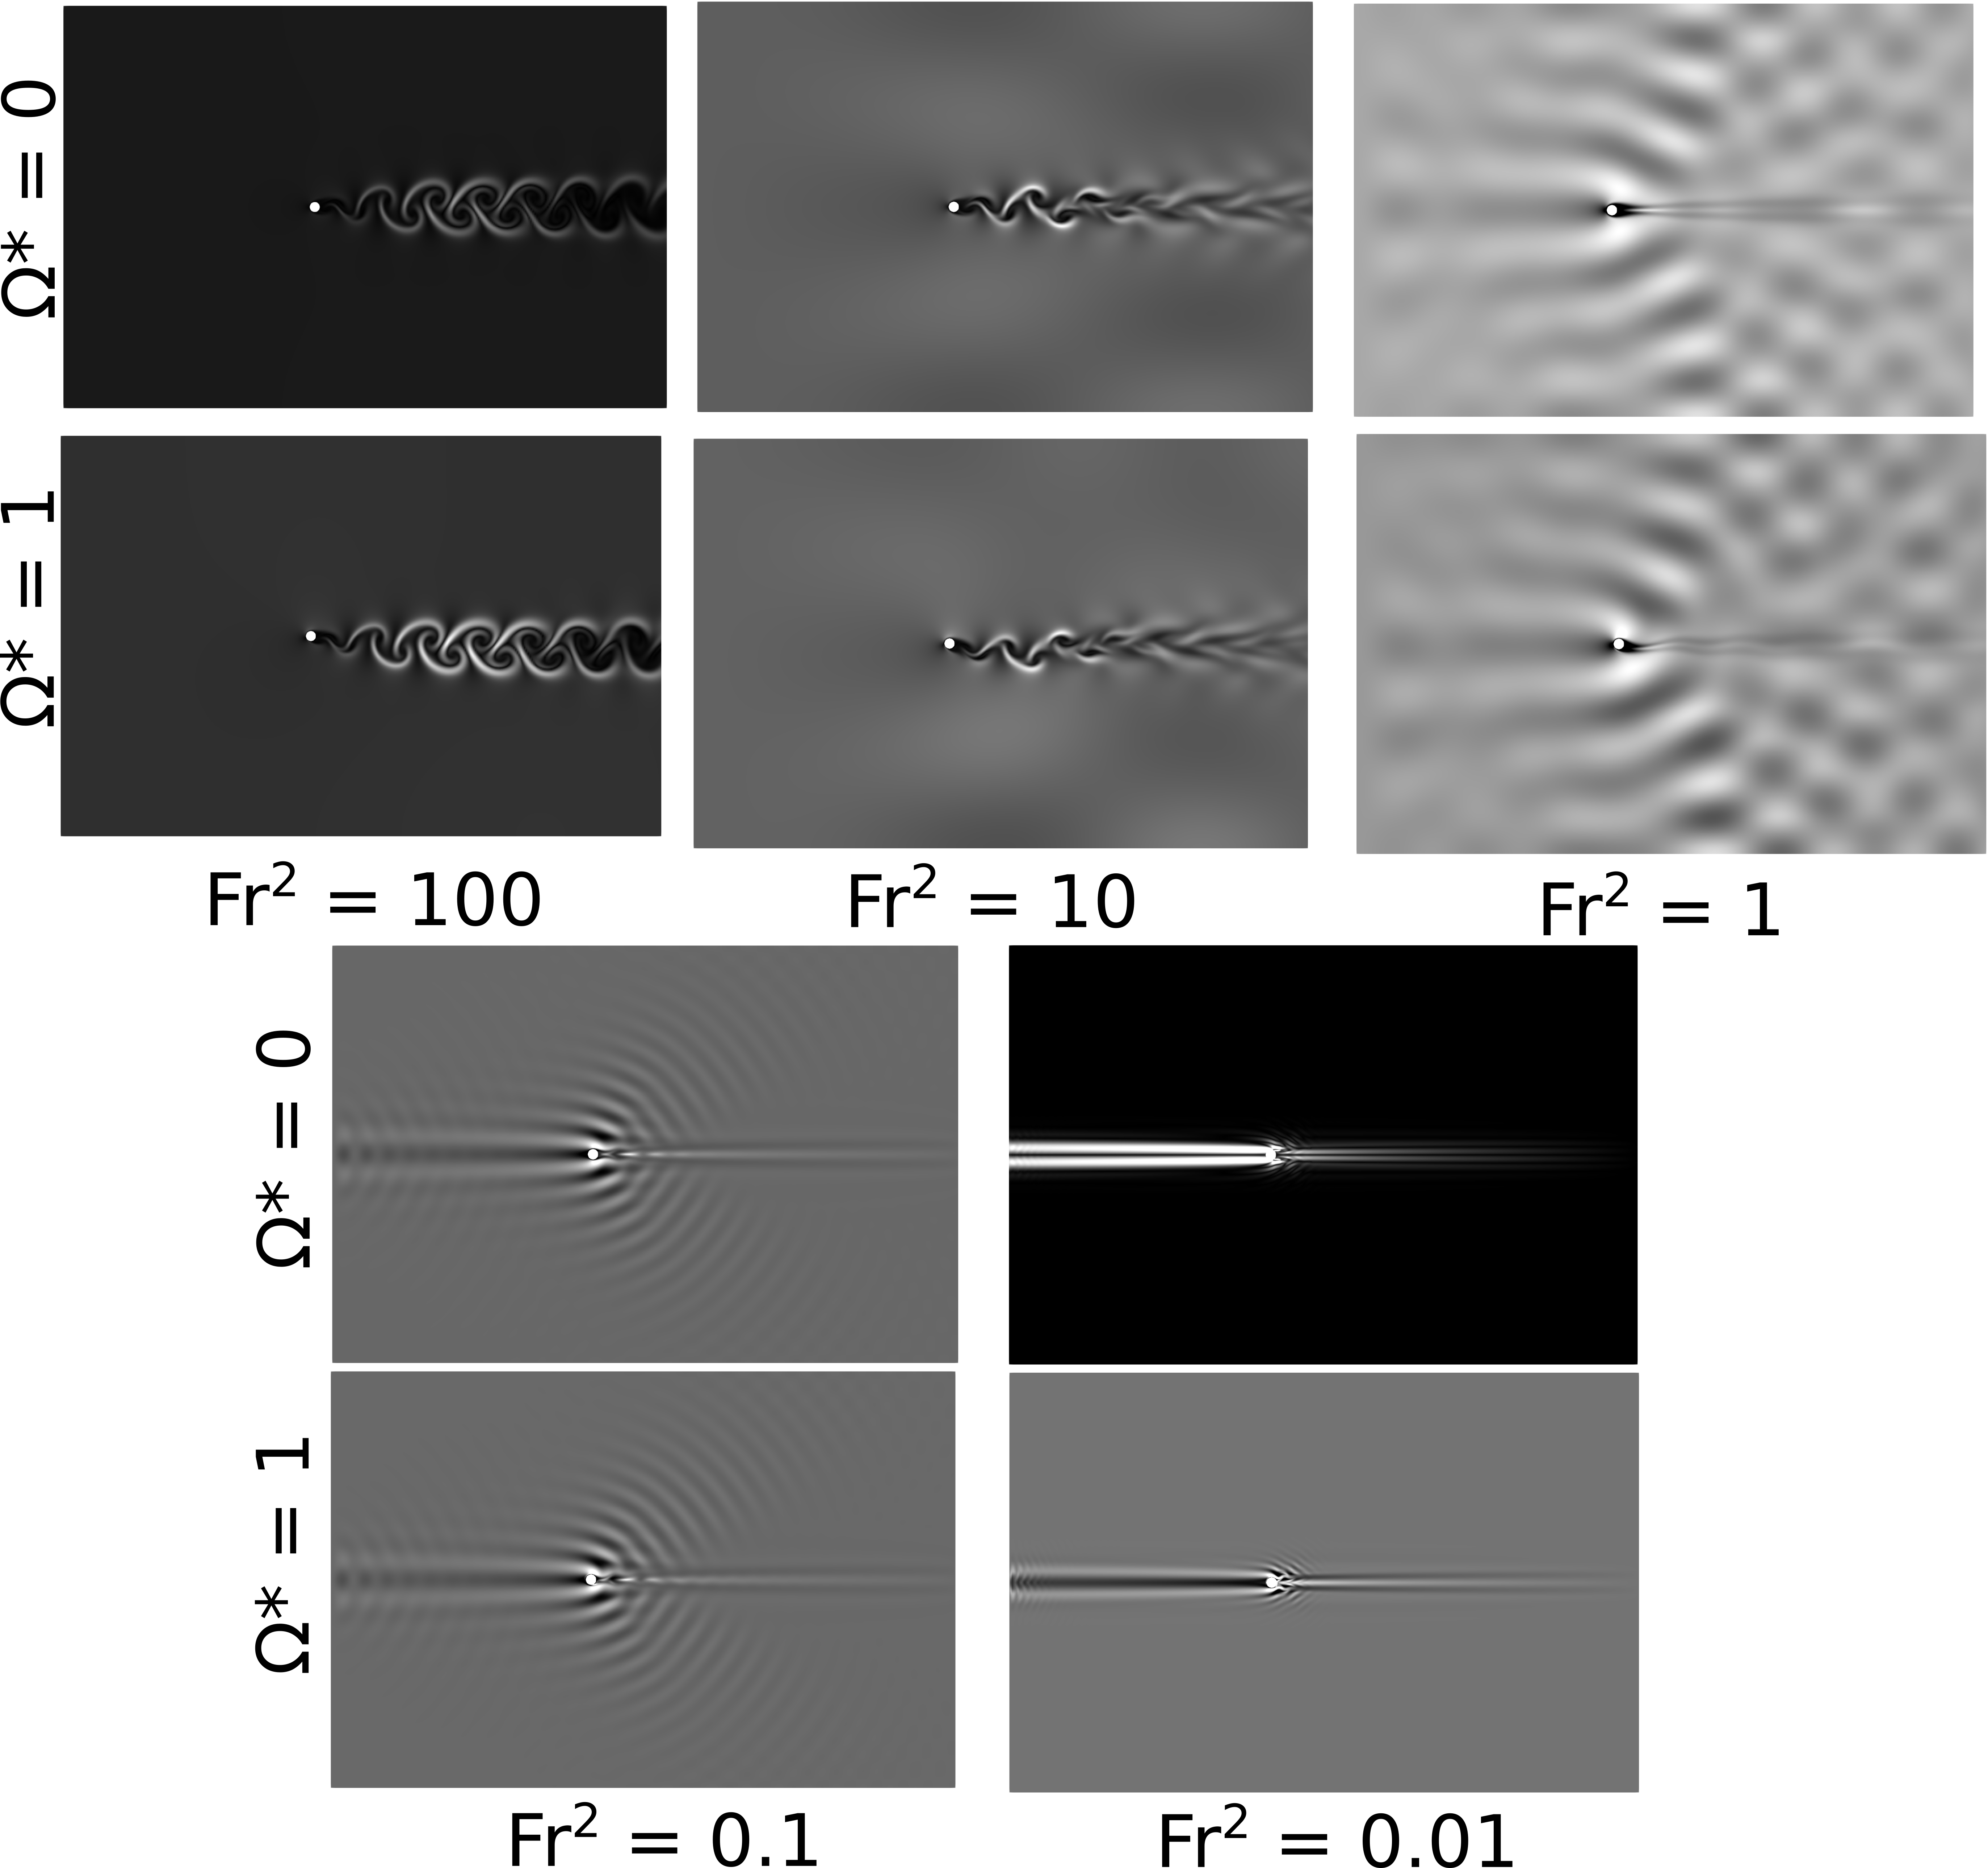
\includegraphics[width=.8\textwidth]{figures/circleschlieren.png}
        \end{figure}
    \end{columns}
\end{frame}

%------------------------------------------------

\begin{frame}{Phase Averaged Drag and Lift}
    \begin{columns}[c]
        \column{.7\textwidth}
        \begin{figure}
            \centering
            \begin{subfigure}[b]{.49\textwidth}
                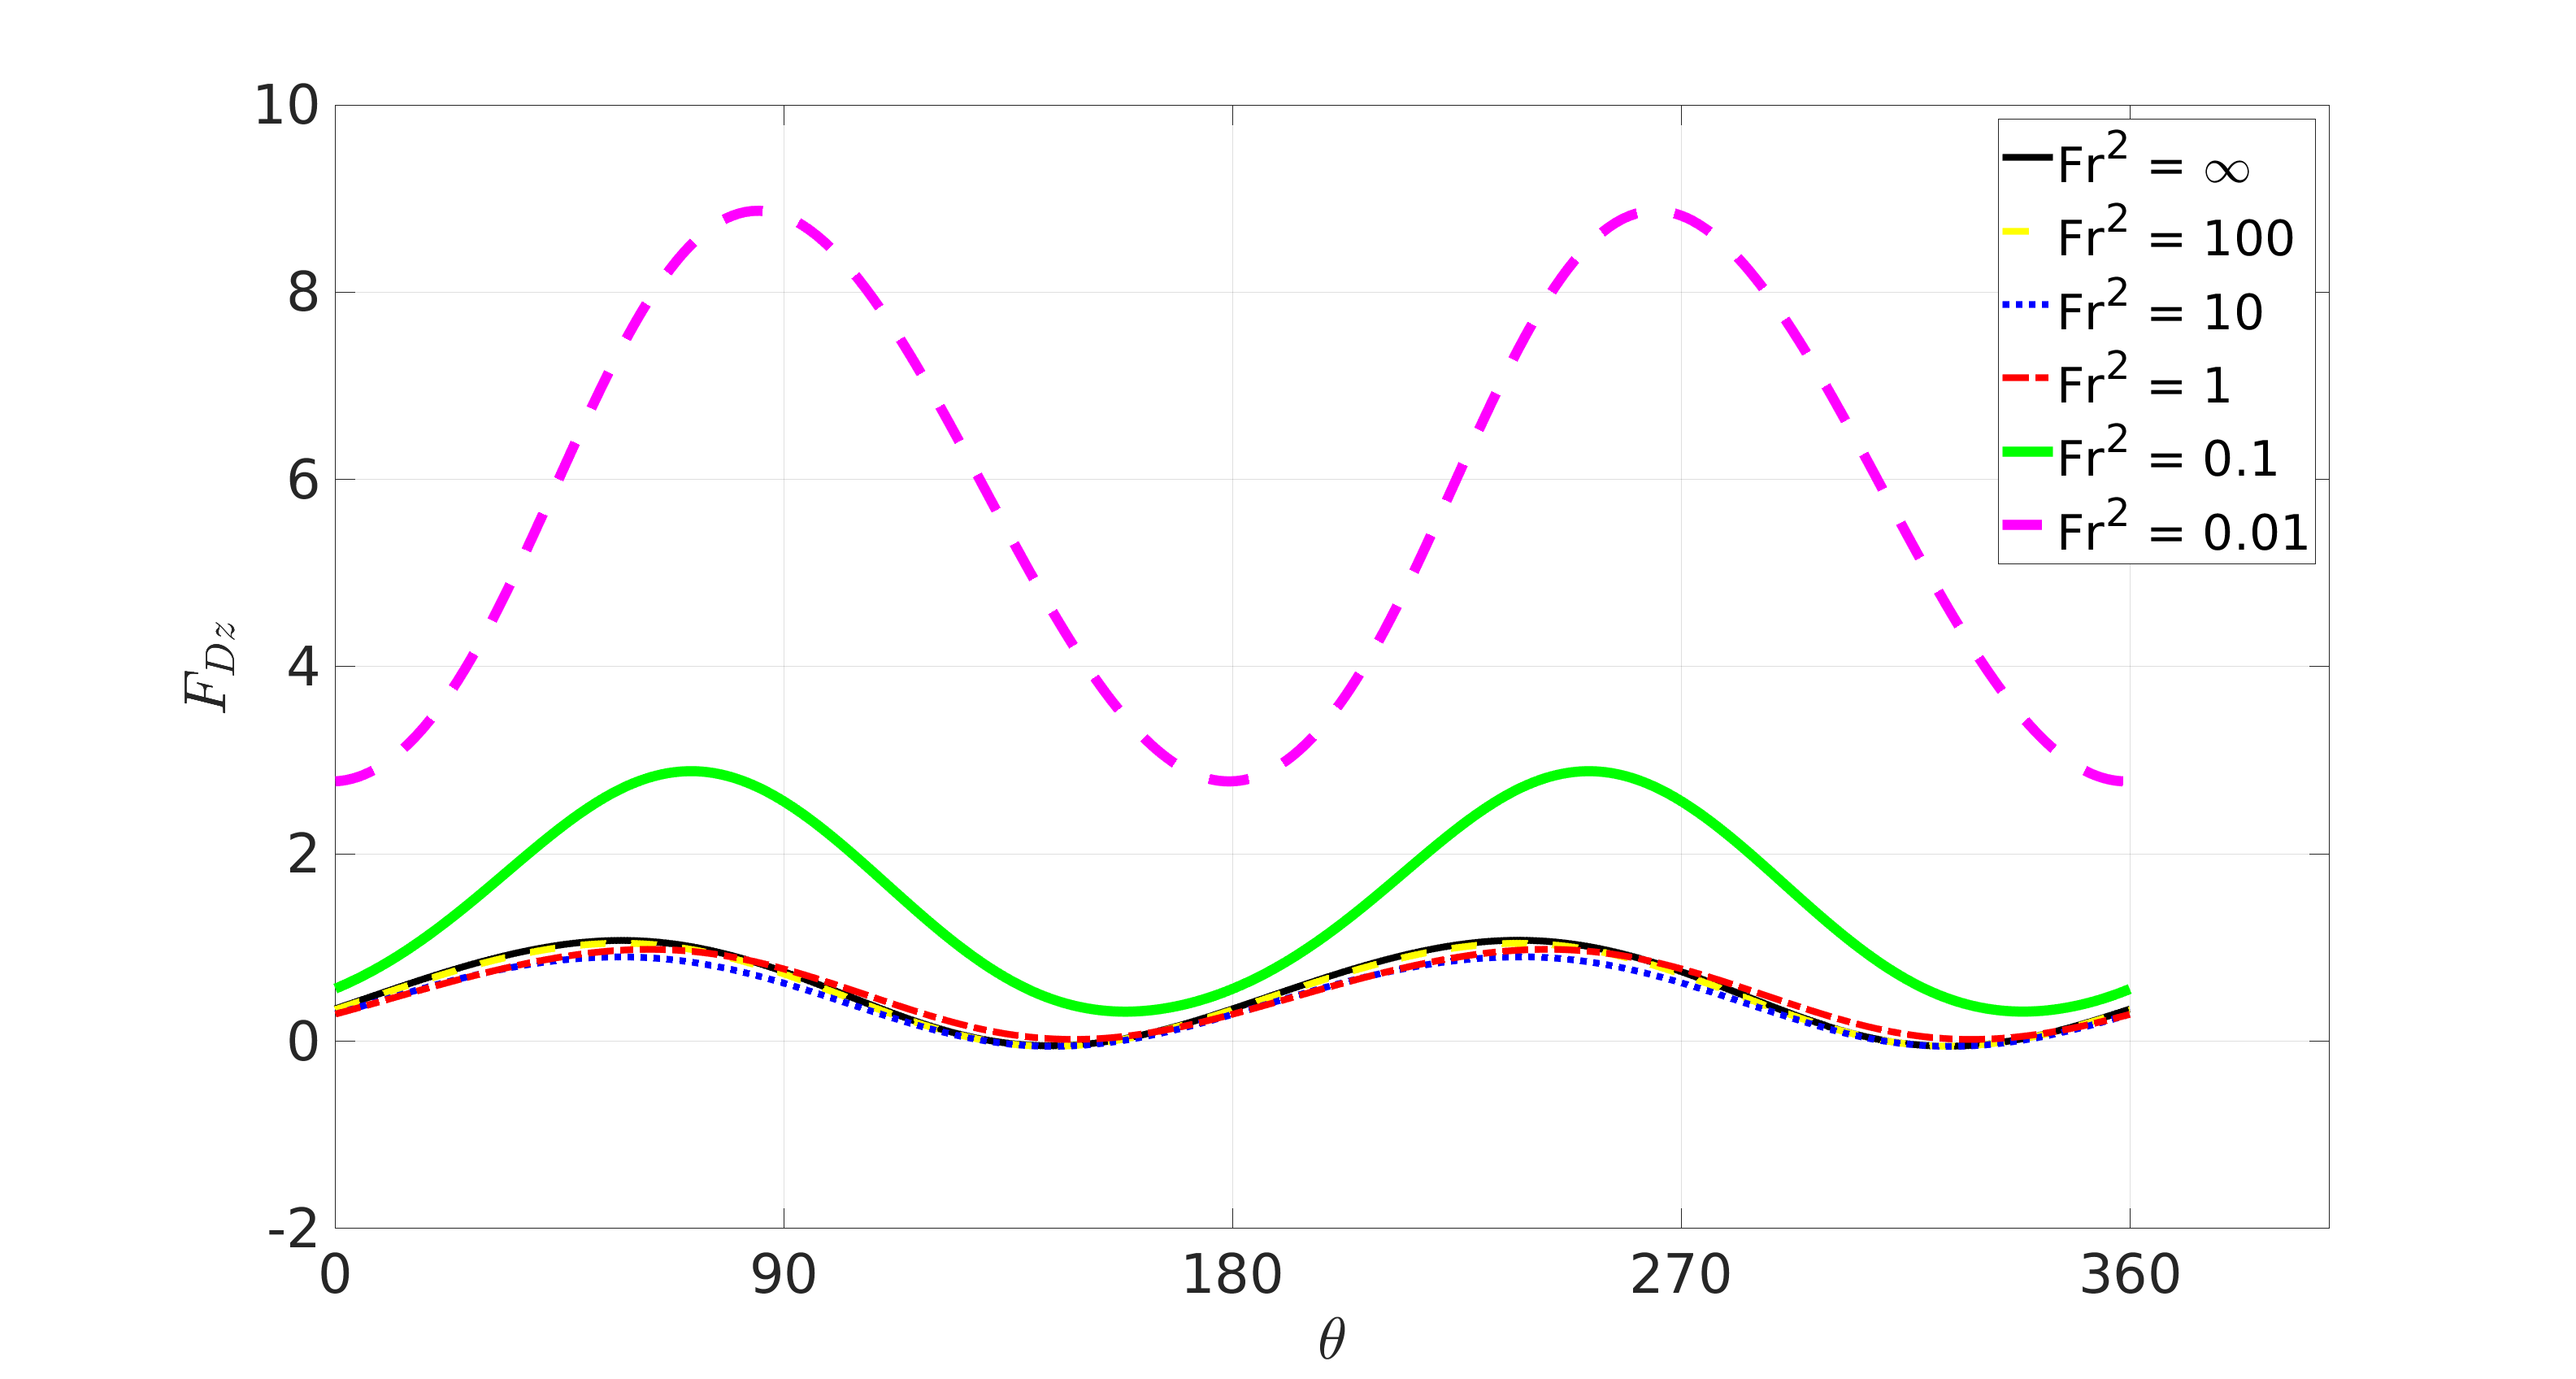
\includegraphics[width=\textwidth]{figures/padrag0p5.pdf}
            \end{subfigure}
            \begin{subfigure}[b]{.49\textwidth}
                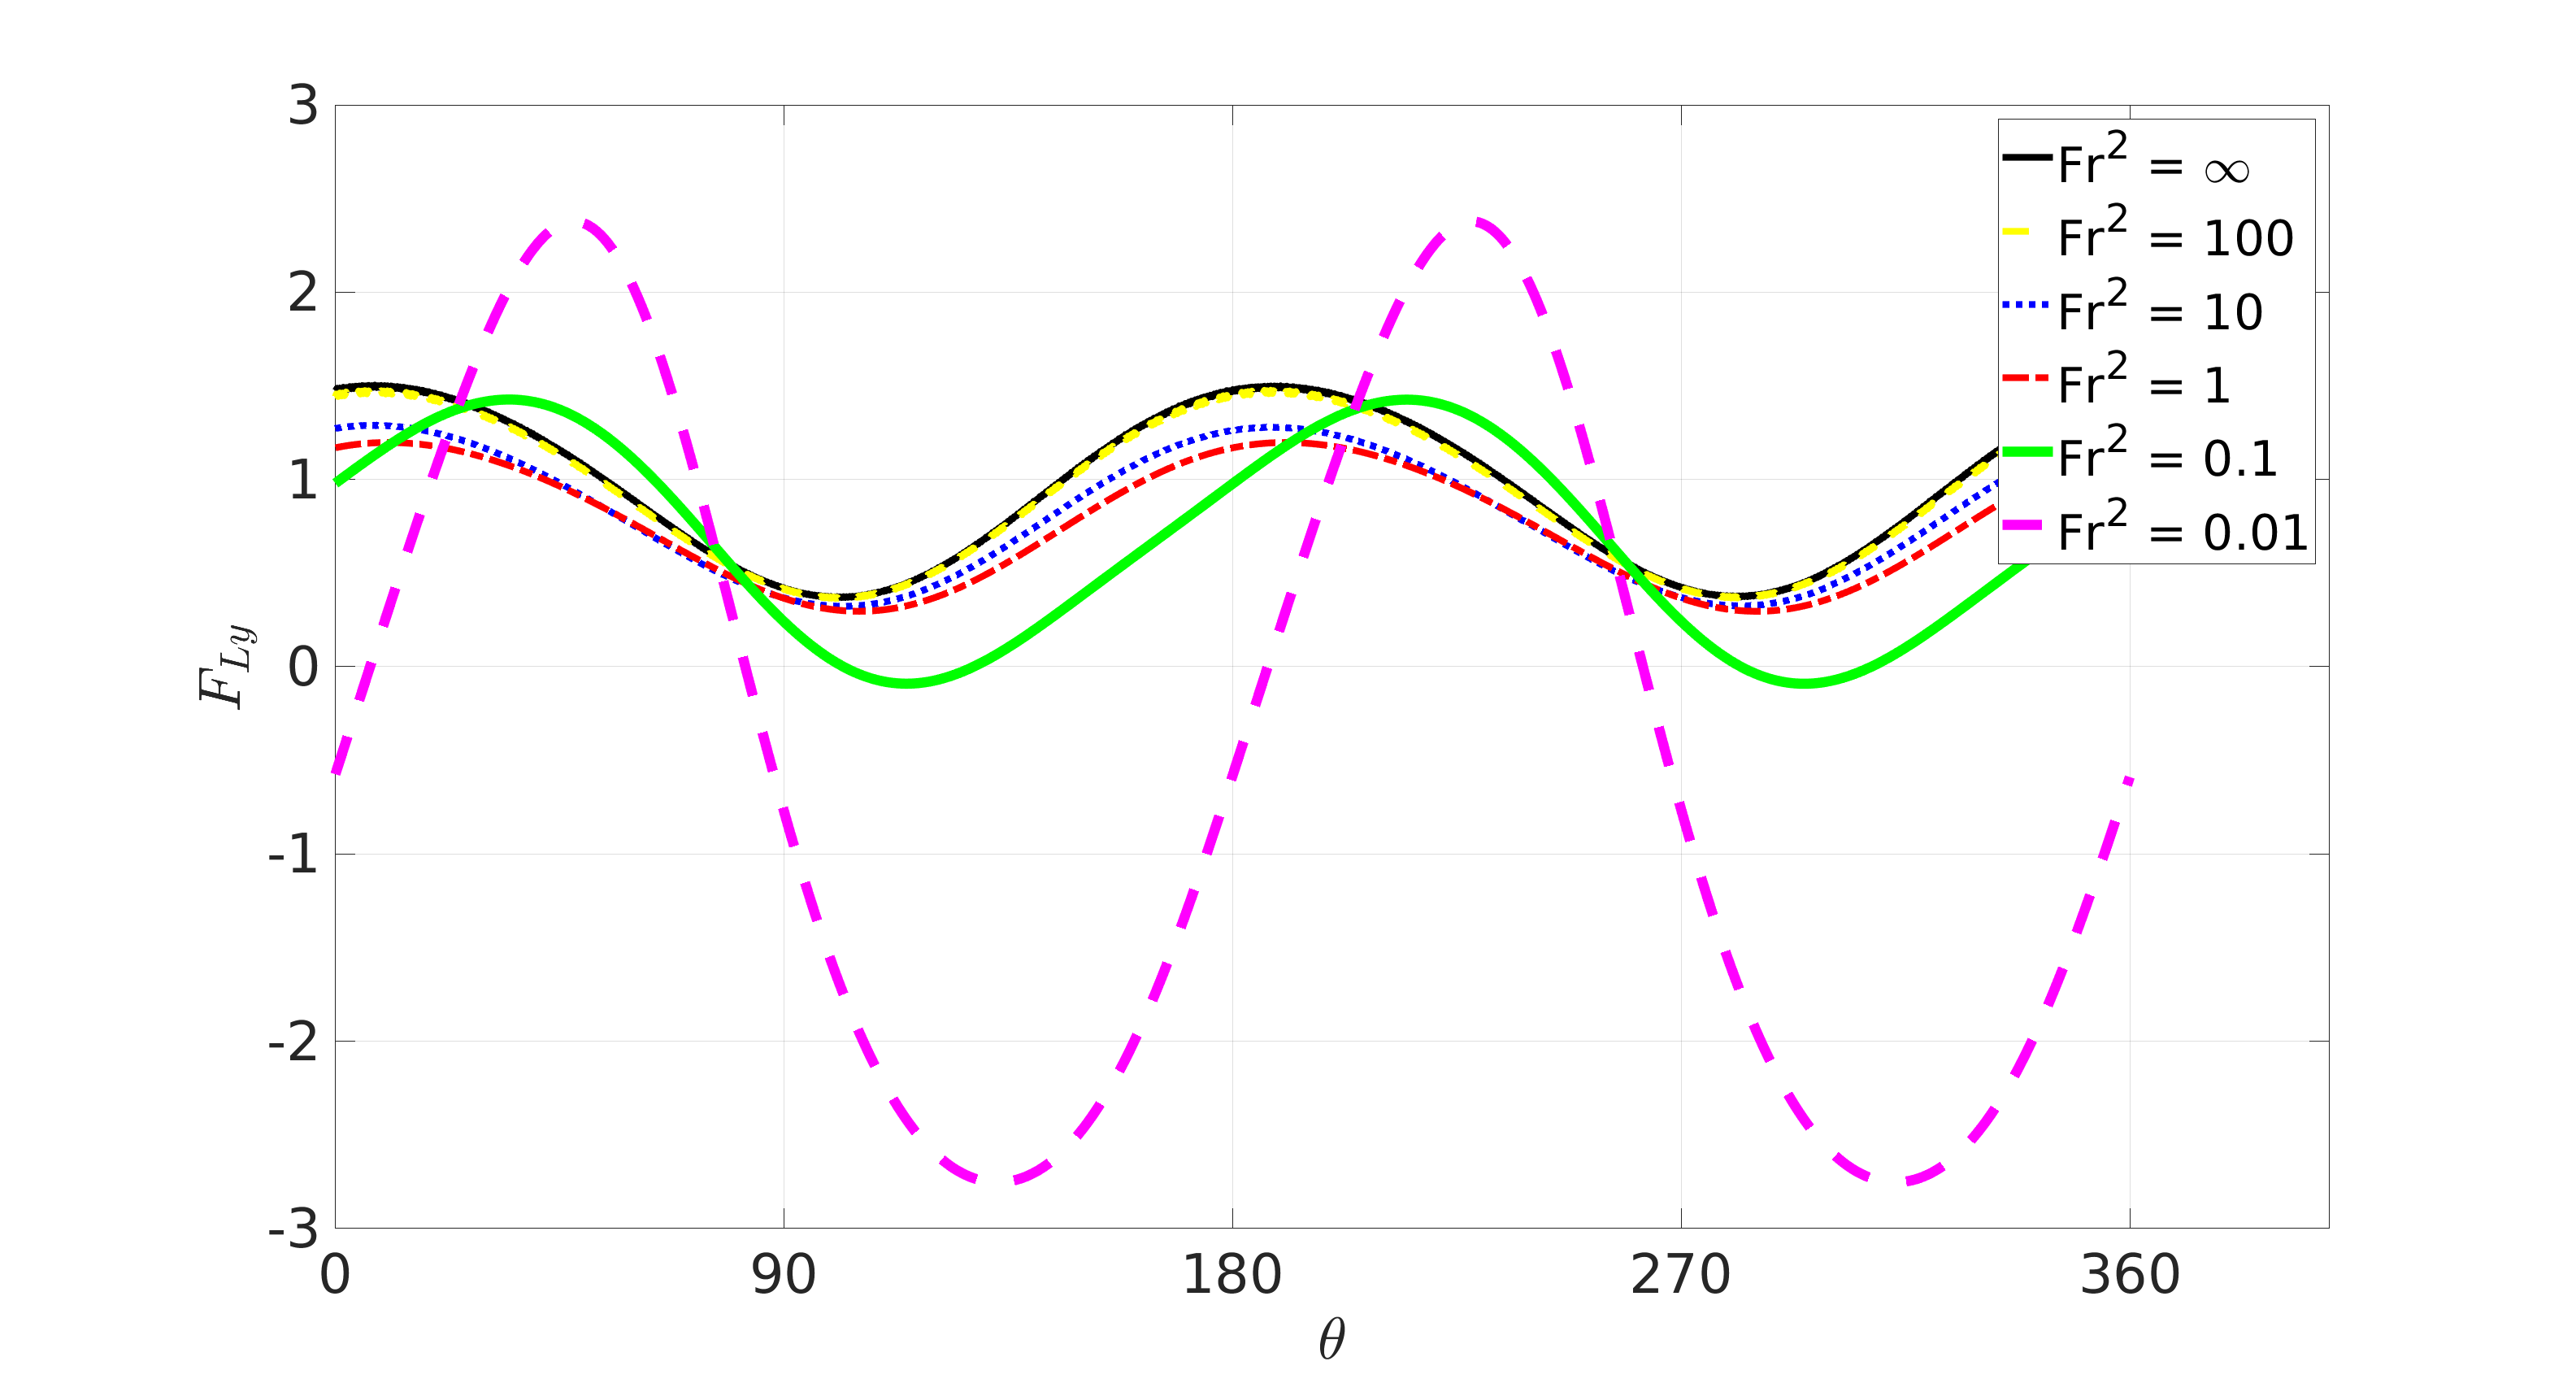
\includegraphics[width=\textwidth]{figures/palift0p5.pdf}
            \end{subfigure}
            \caption{Phase-averaged drag and lift for $AR = 0.5$}
        \end{figure}
        \vspace{-10pt}
        \begin{figure}
            \centering
            \begin{subfigure}[b]{.49\textwidth}
                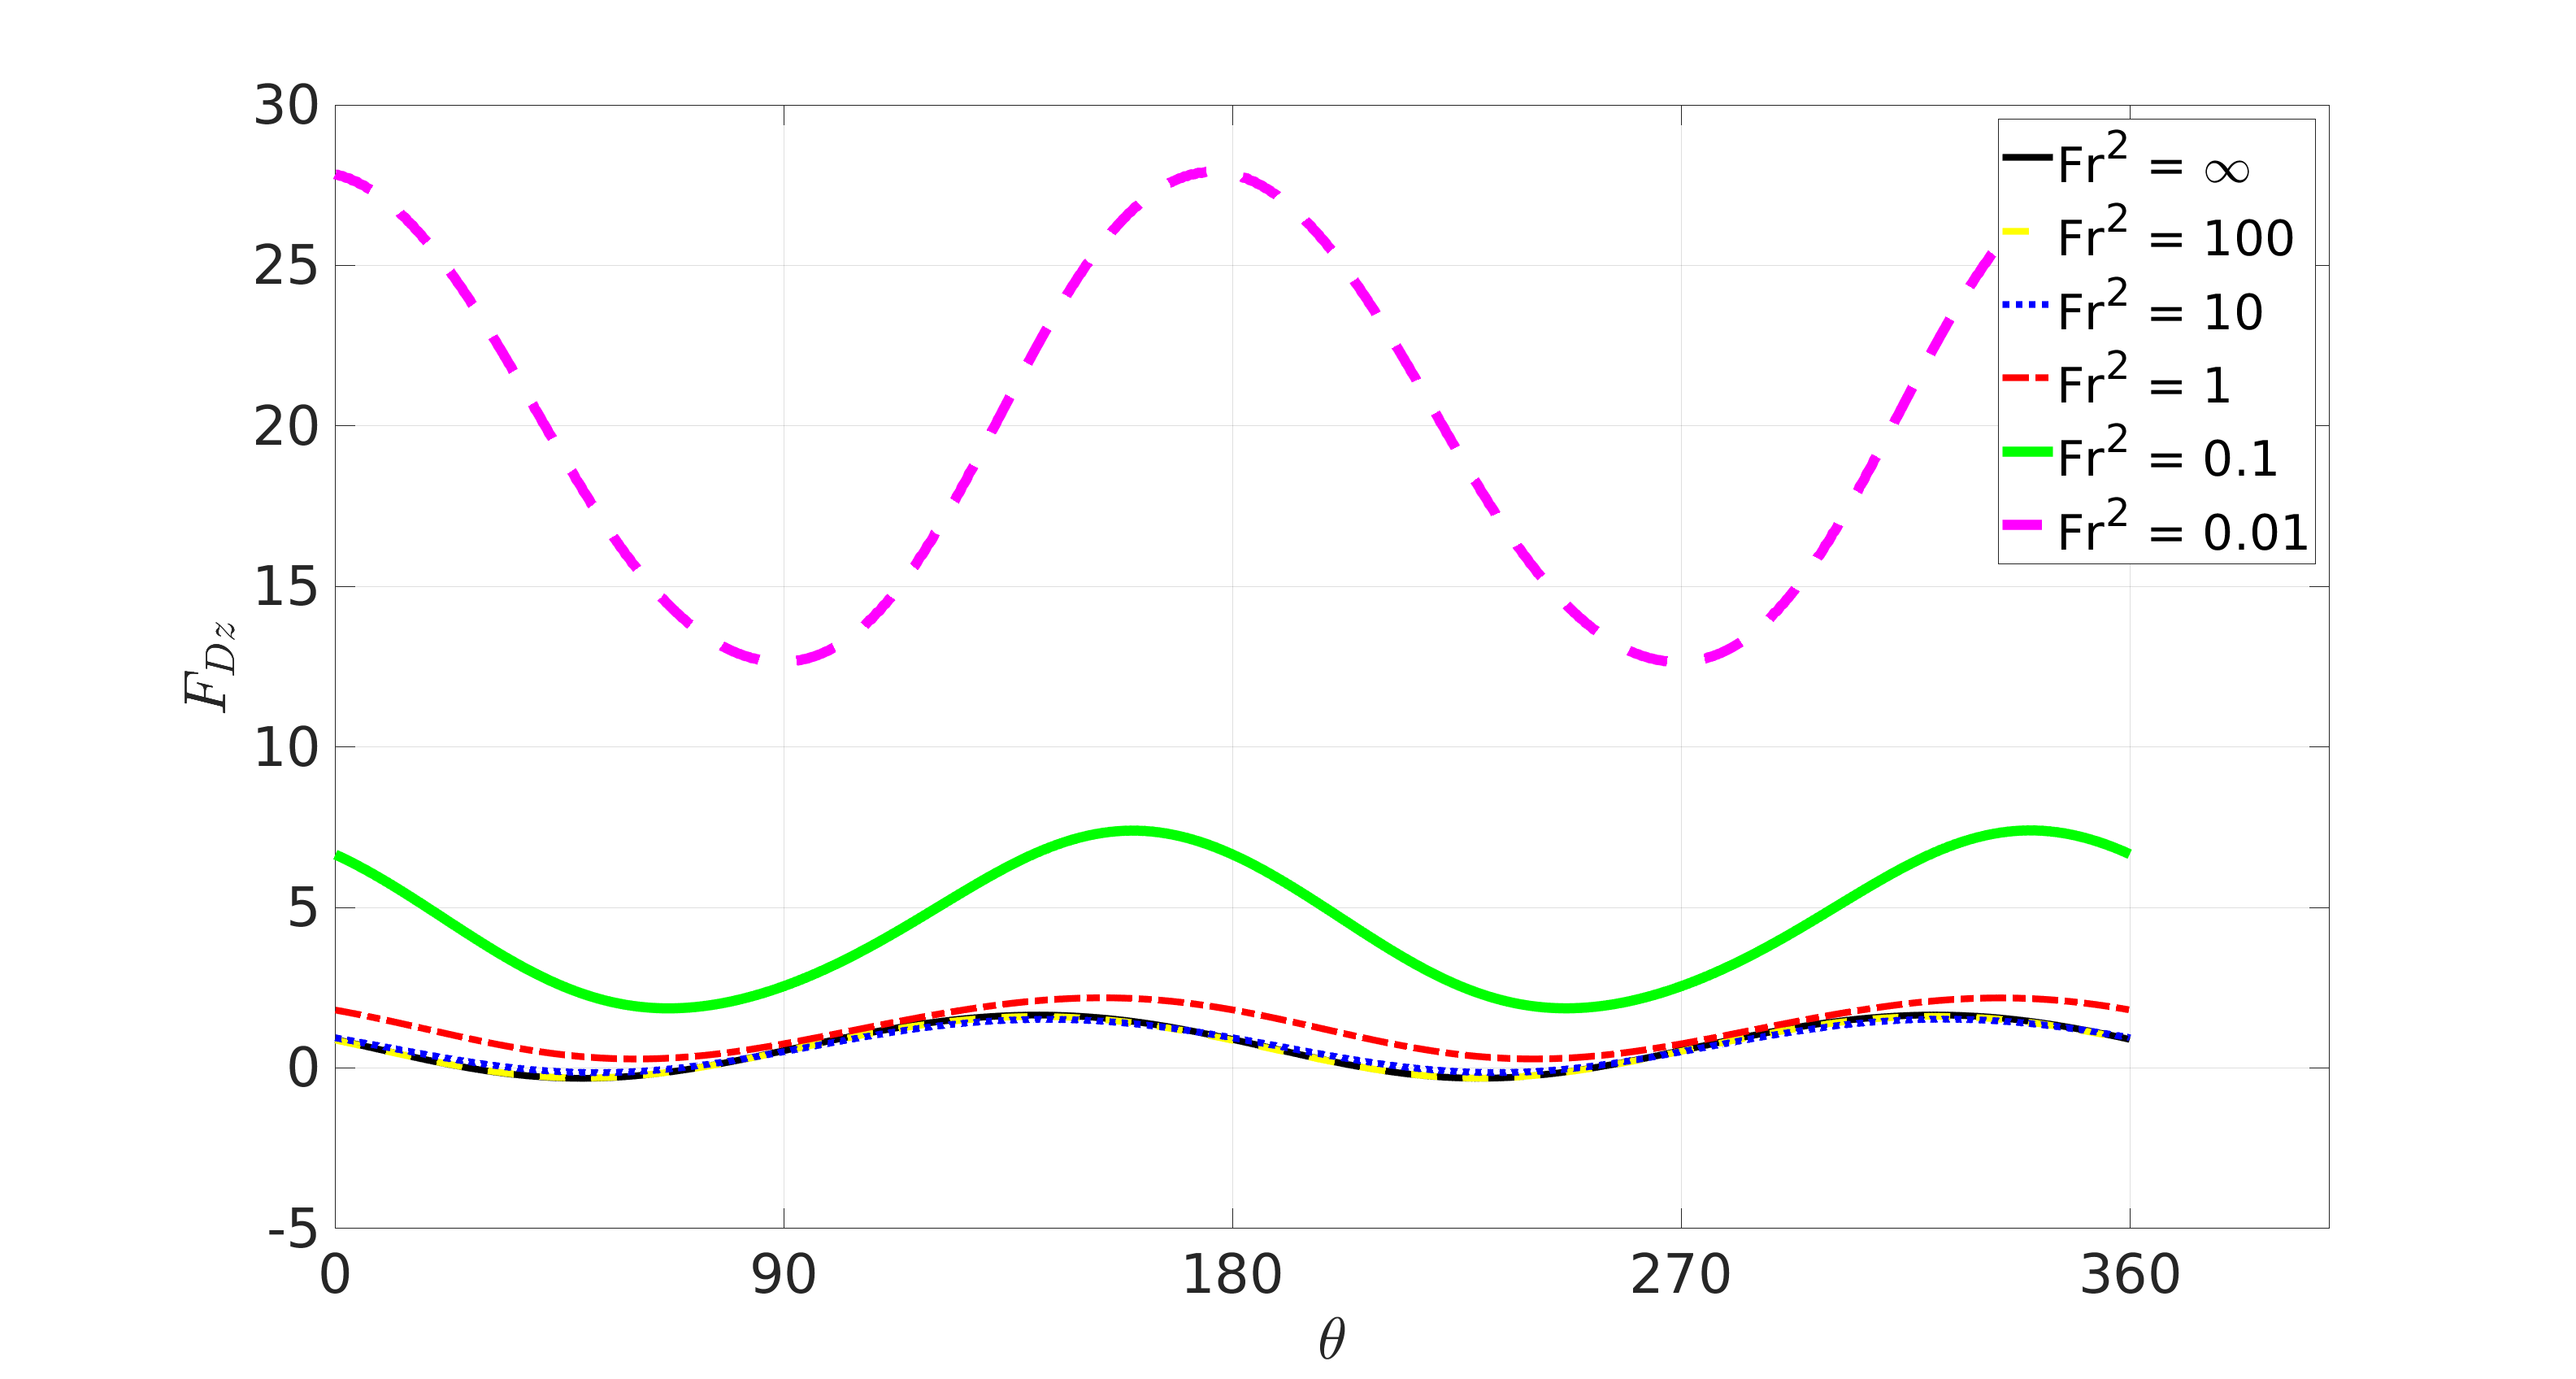
\includegraphics[width=\textwidth]{figures/padrag1p5.pdf}
            \end{subfigure}
            \begin{subfigure}[b]{.49\textwidth}
                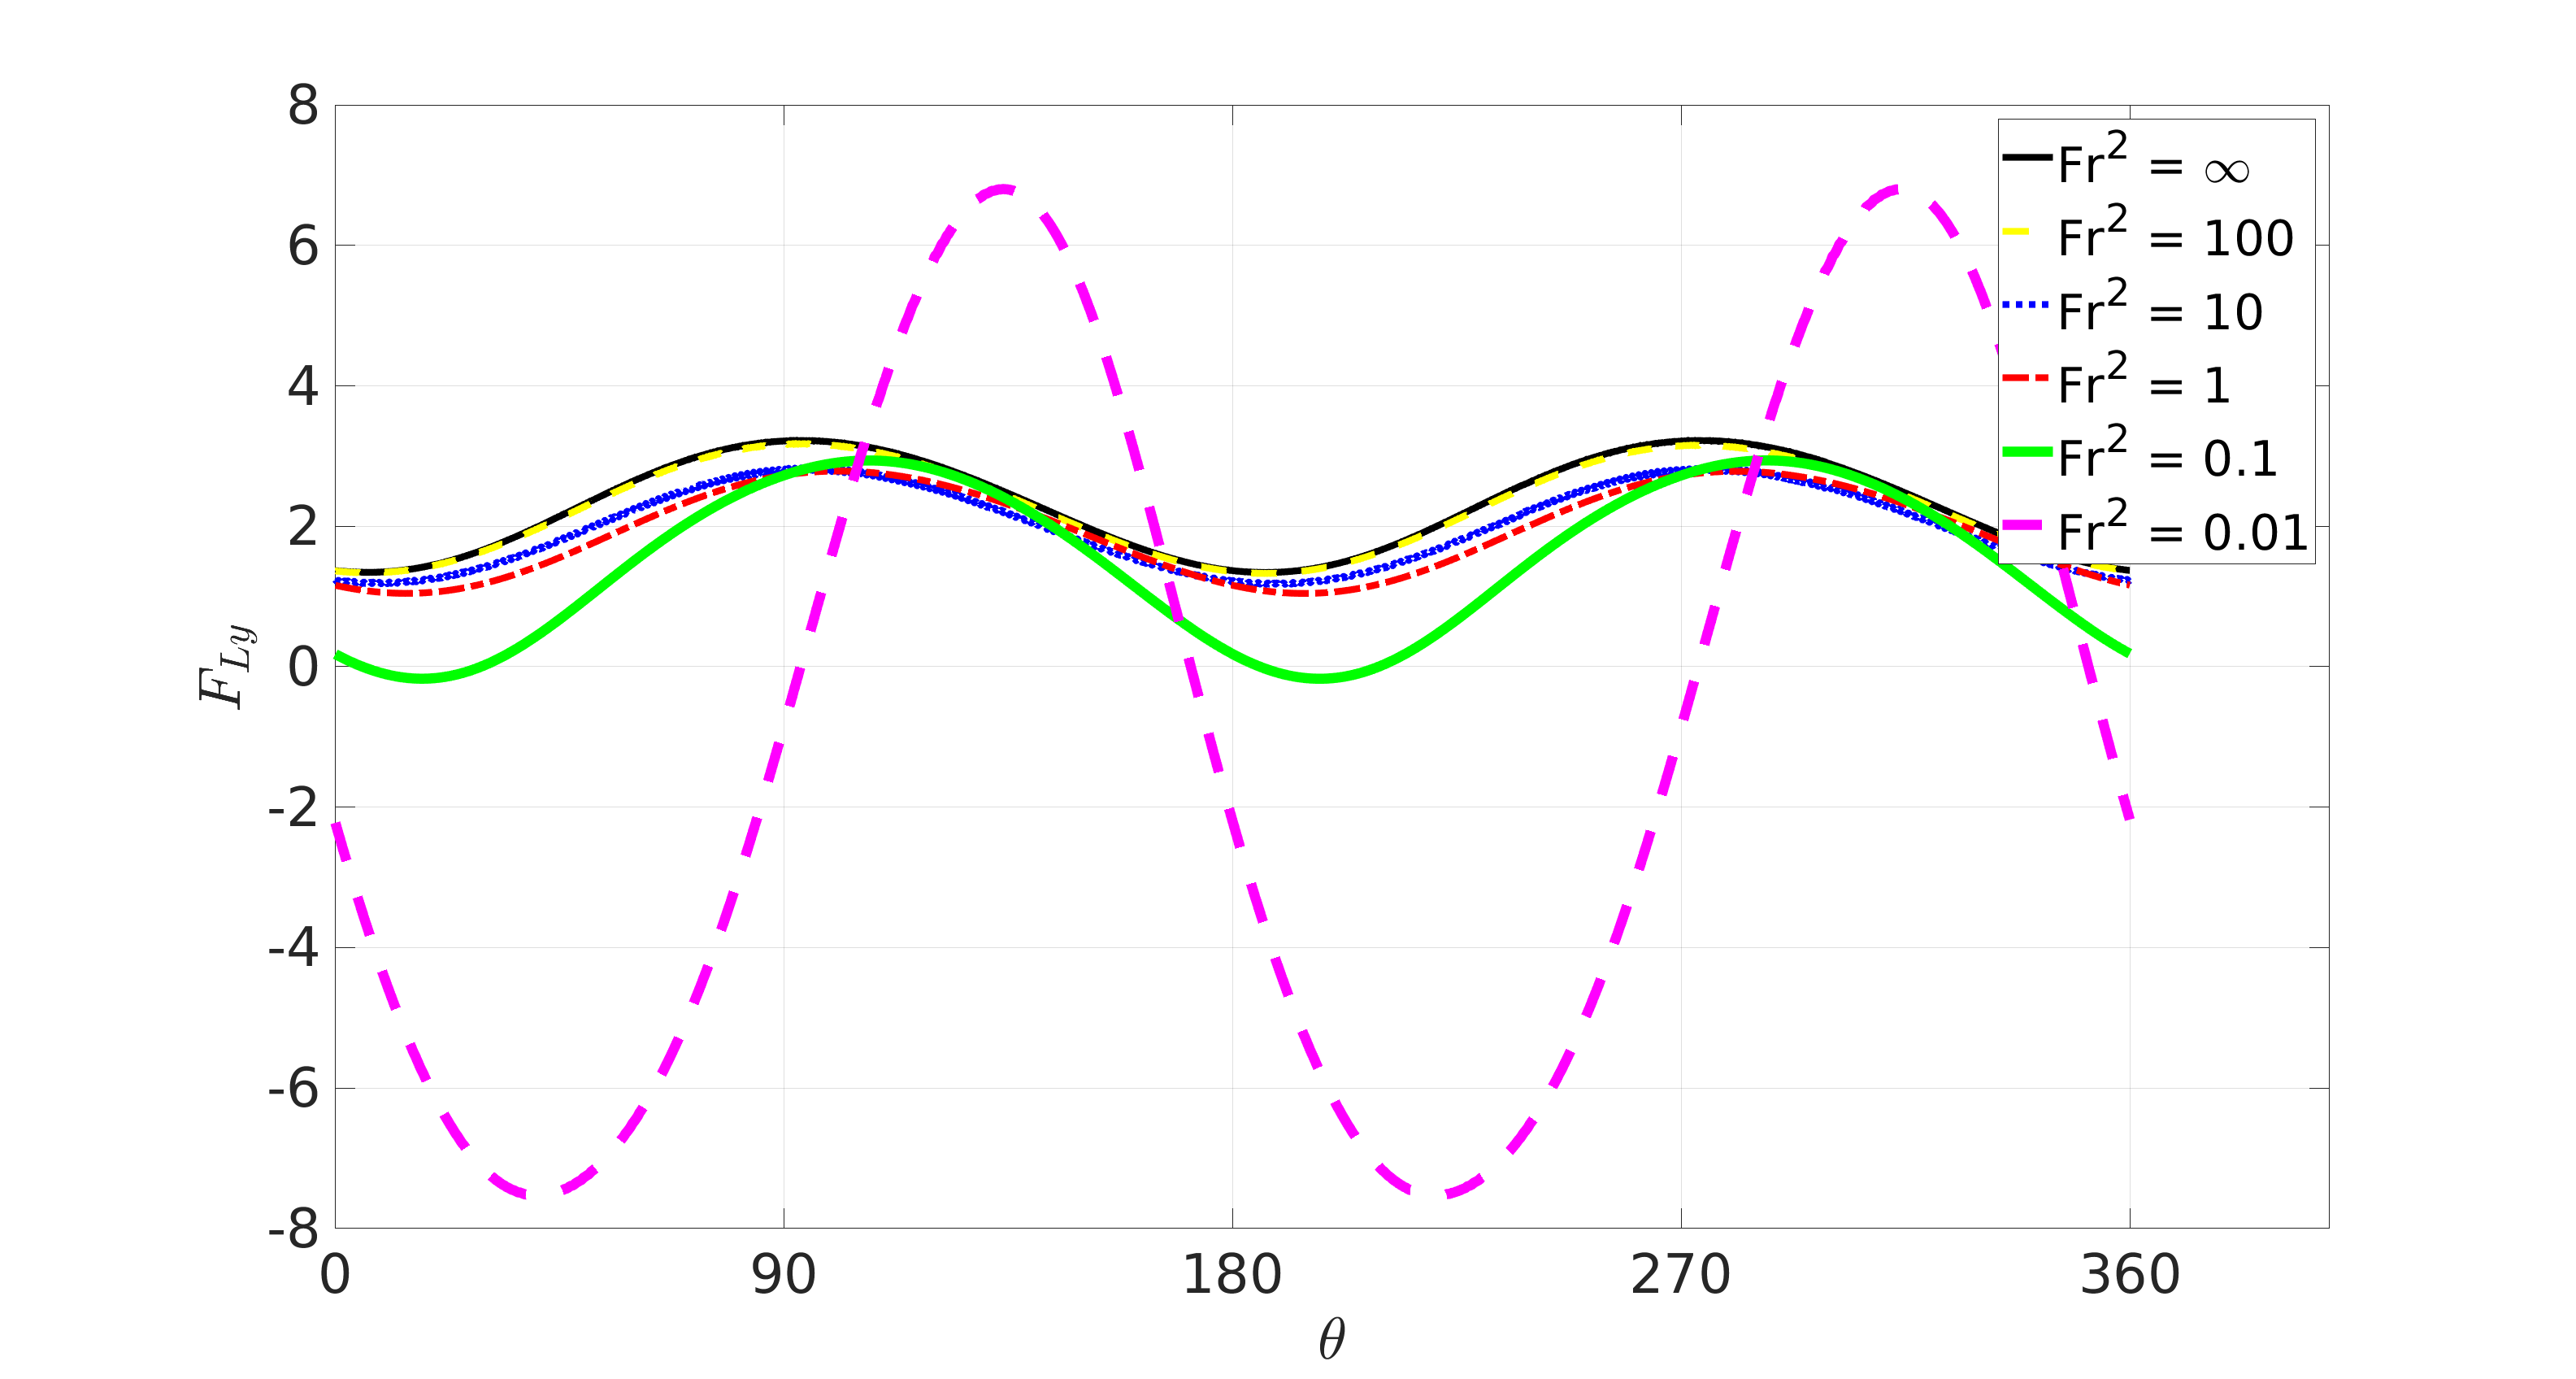
\includegraphics[width=\textwidth]{figures/palift1p5.pdf}
            \end{subfigure}
            \caption{Phase-averaged drag and lift for $AR = 1.5$}
        \end{figure}
        \column{.3\textwidth}

\end{columns}
\end{frame}

%------------------------------------------------

\begin{frame}{Ellipse Schlieren Plots}
    \begin{columns}[c]
        \column{.4\textwidth}
        \begin{itemize}
            \item Same large-scale flow structures as in the circle cases are present
            \item Unsteady internal gravity waves manifest themselves in the cases of $Fr^2 = 0.1, 0.01$ 
            \item Internal gravity wave reflection off domain boundaries is present in the $Fr^2 = 0.01$ case
        \end{itemize}
        \column{.1\textwidth}
        \begin{tikzpicture}
            \draw (0,0) -- (0,0);
            \node at (2,2) {\rotatebox{90}{$AR = 0.5$}};           
            \node at (2,-2) {\rotatebox{90}{$AR = 1.5$}};           
        \end{tikzpicture}
        
        \column{.5\textwidth}
        \vspace{-10pt}
        \begin{figure}
            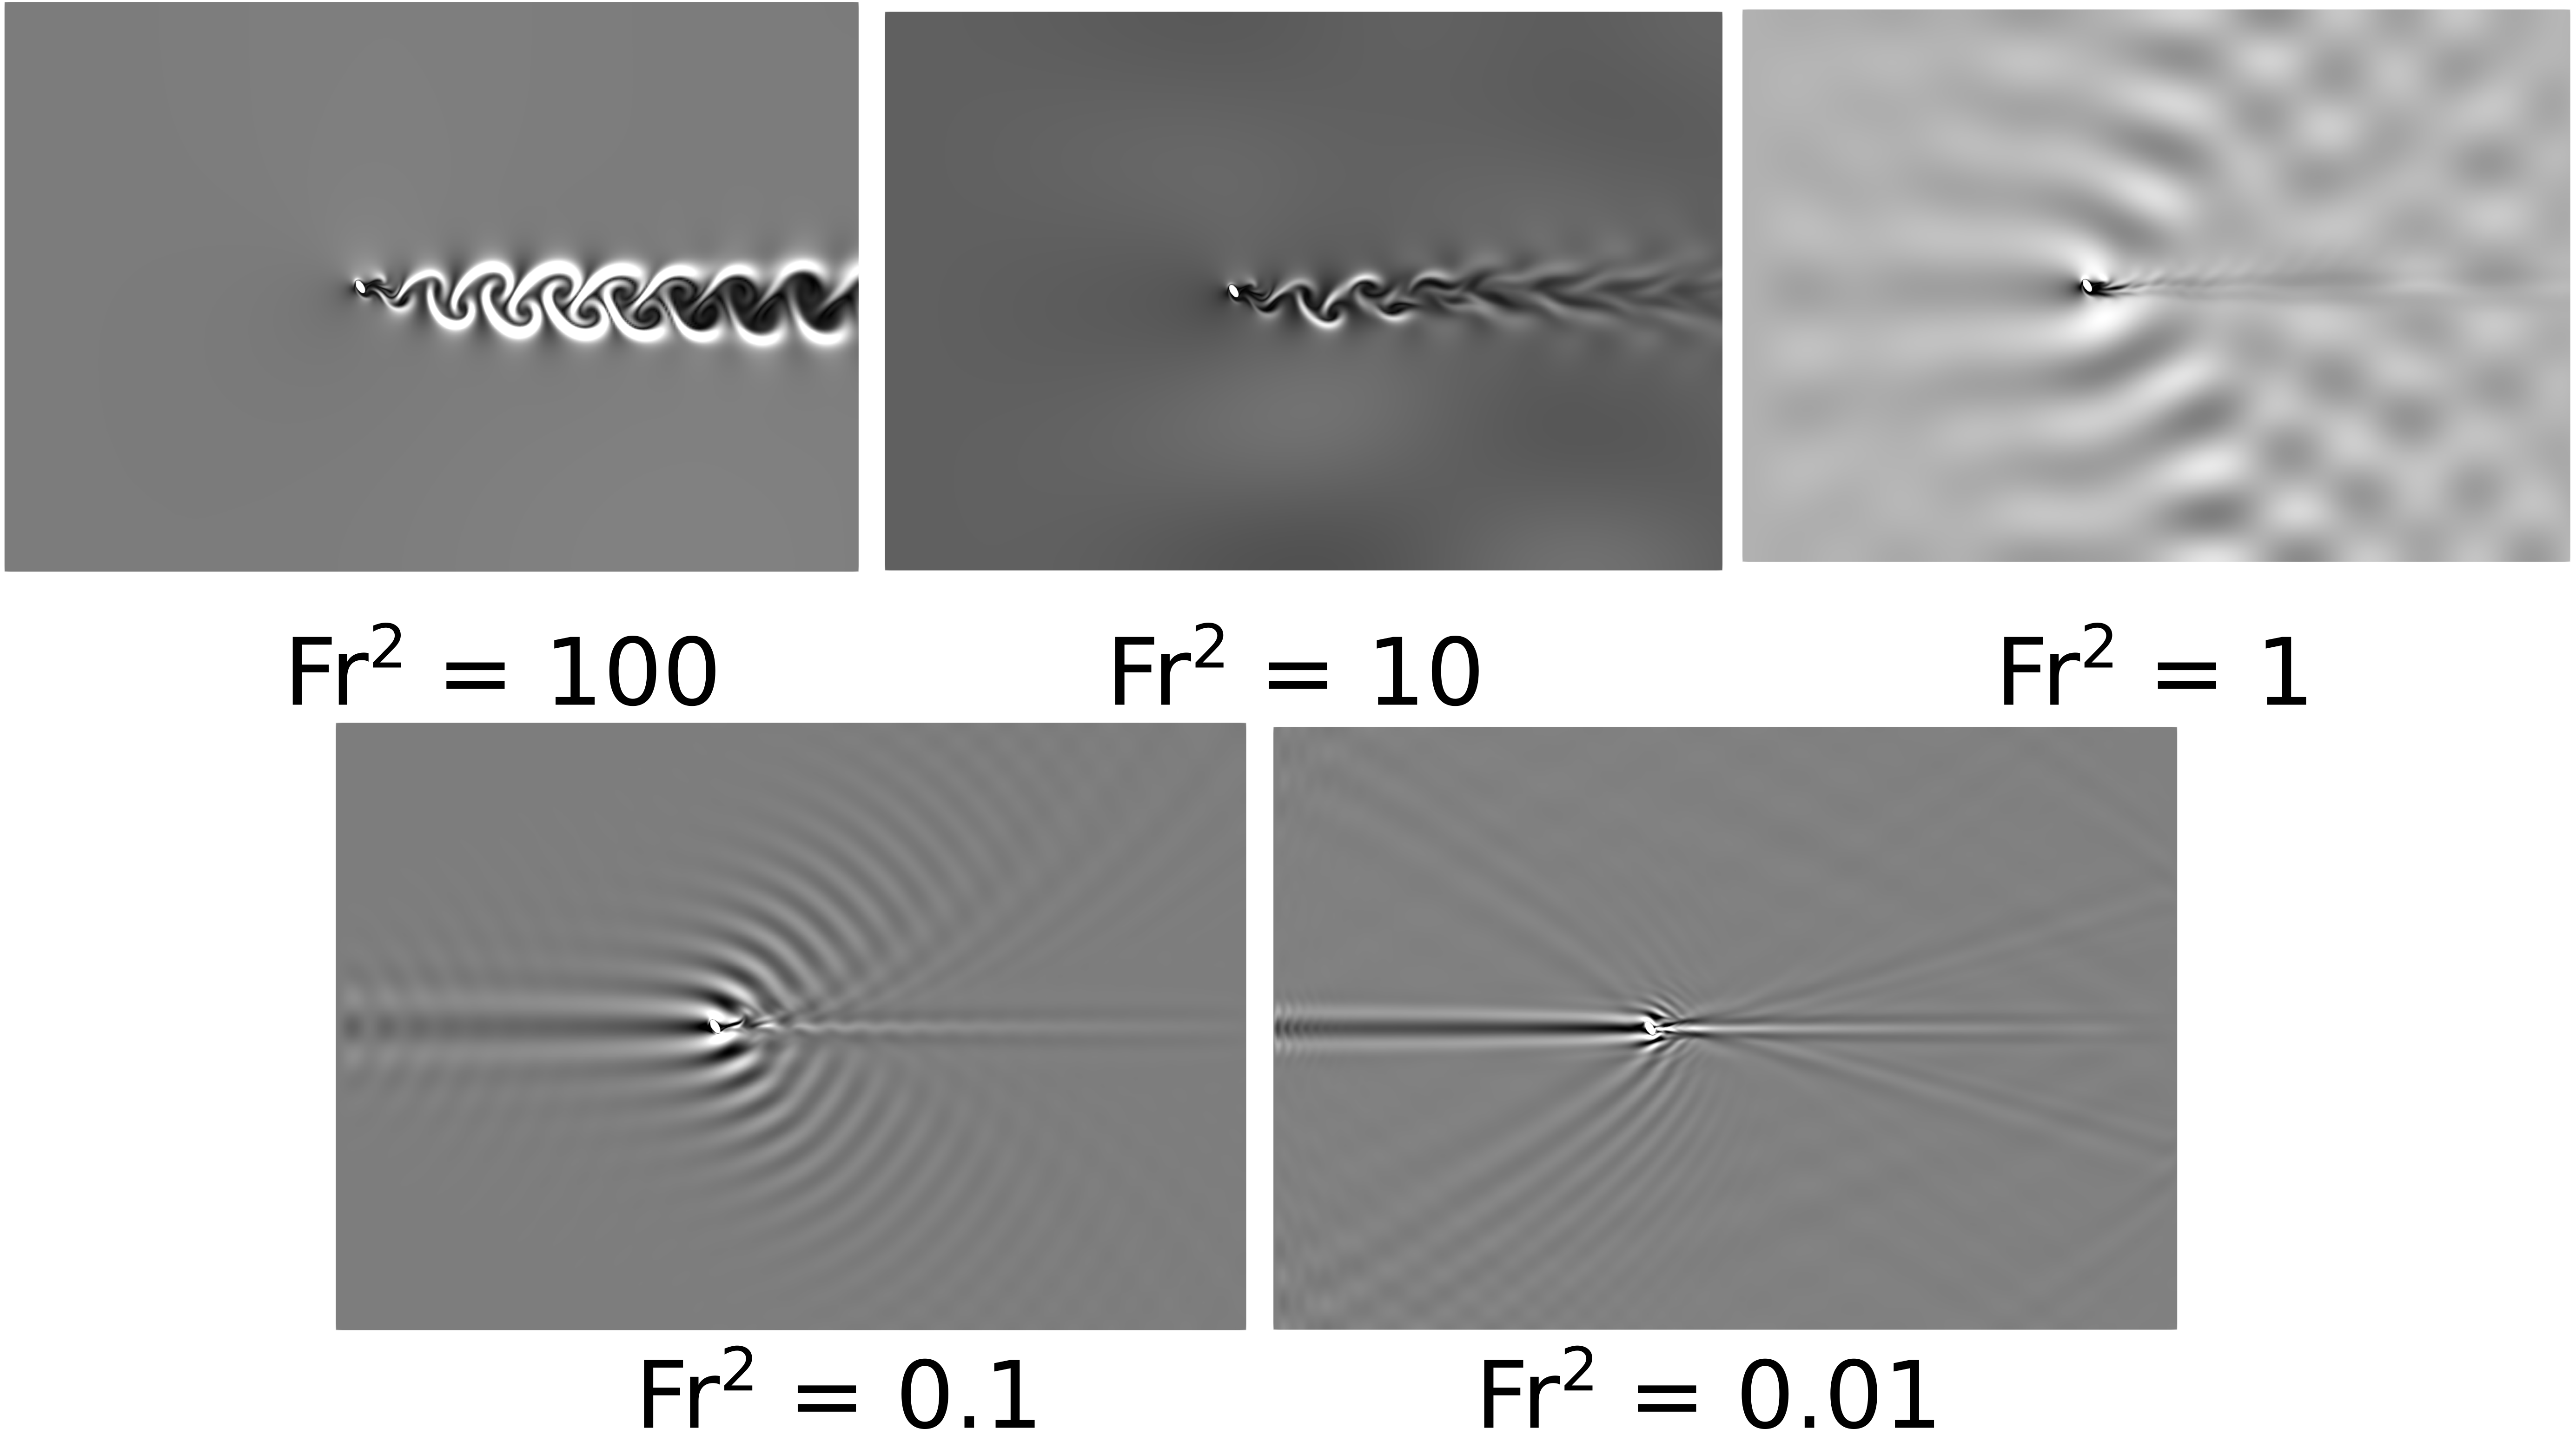
\includegraphics[width=.8\textwidth]{figures/schlierenar0p5.png}
%           \caption*{$AR = 0.5$ Schlieren}
        \end{figure}
        \vspace{-10pt}
        \makebox[\linewidth]{\rule{\textwidth}{0.4pt}}
        \begin{figure}
            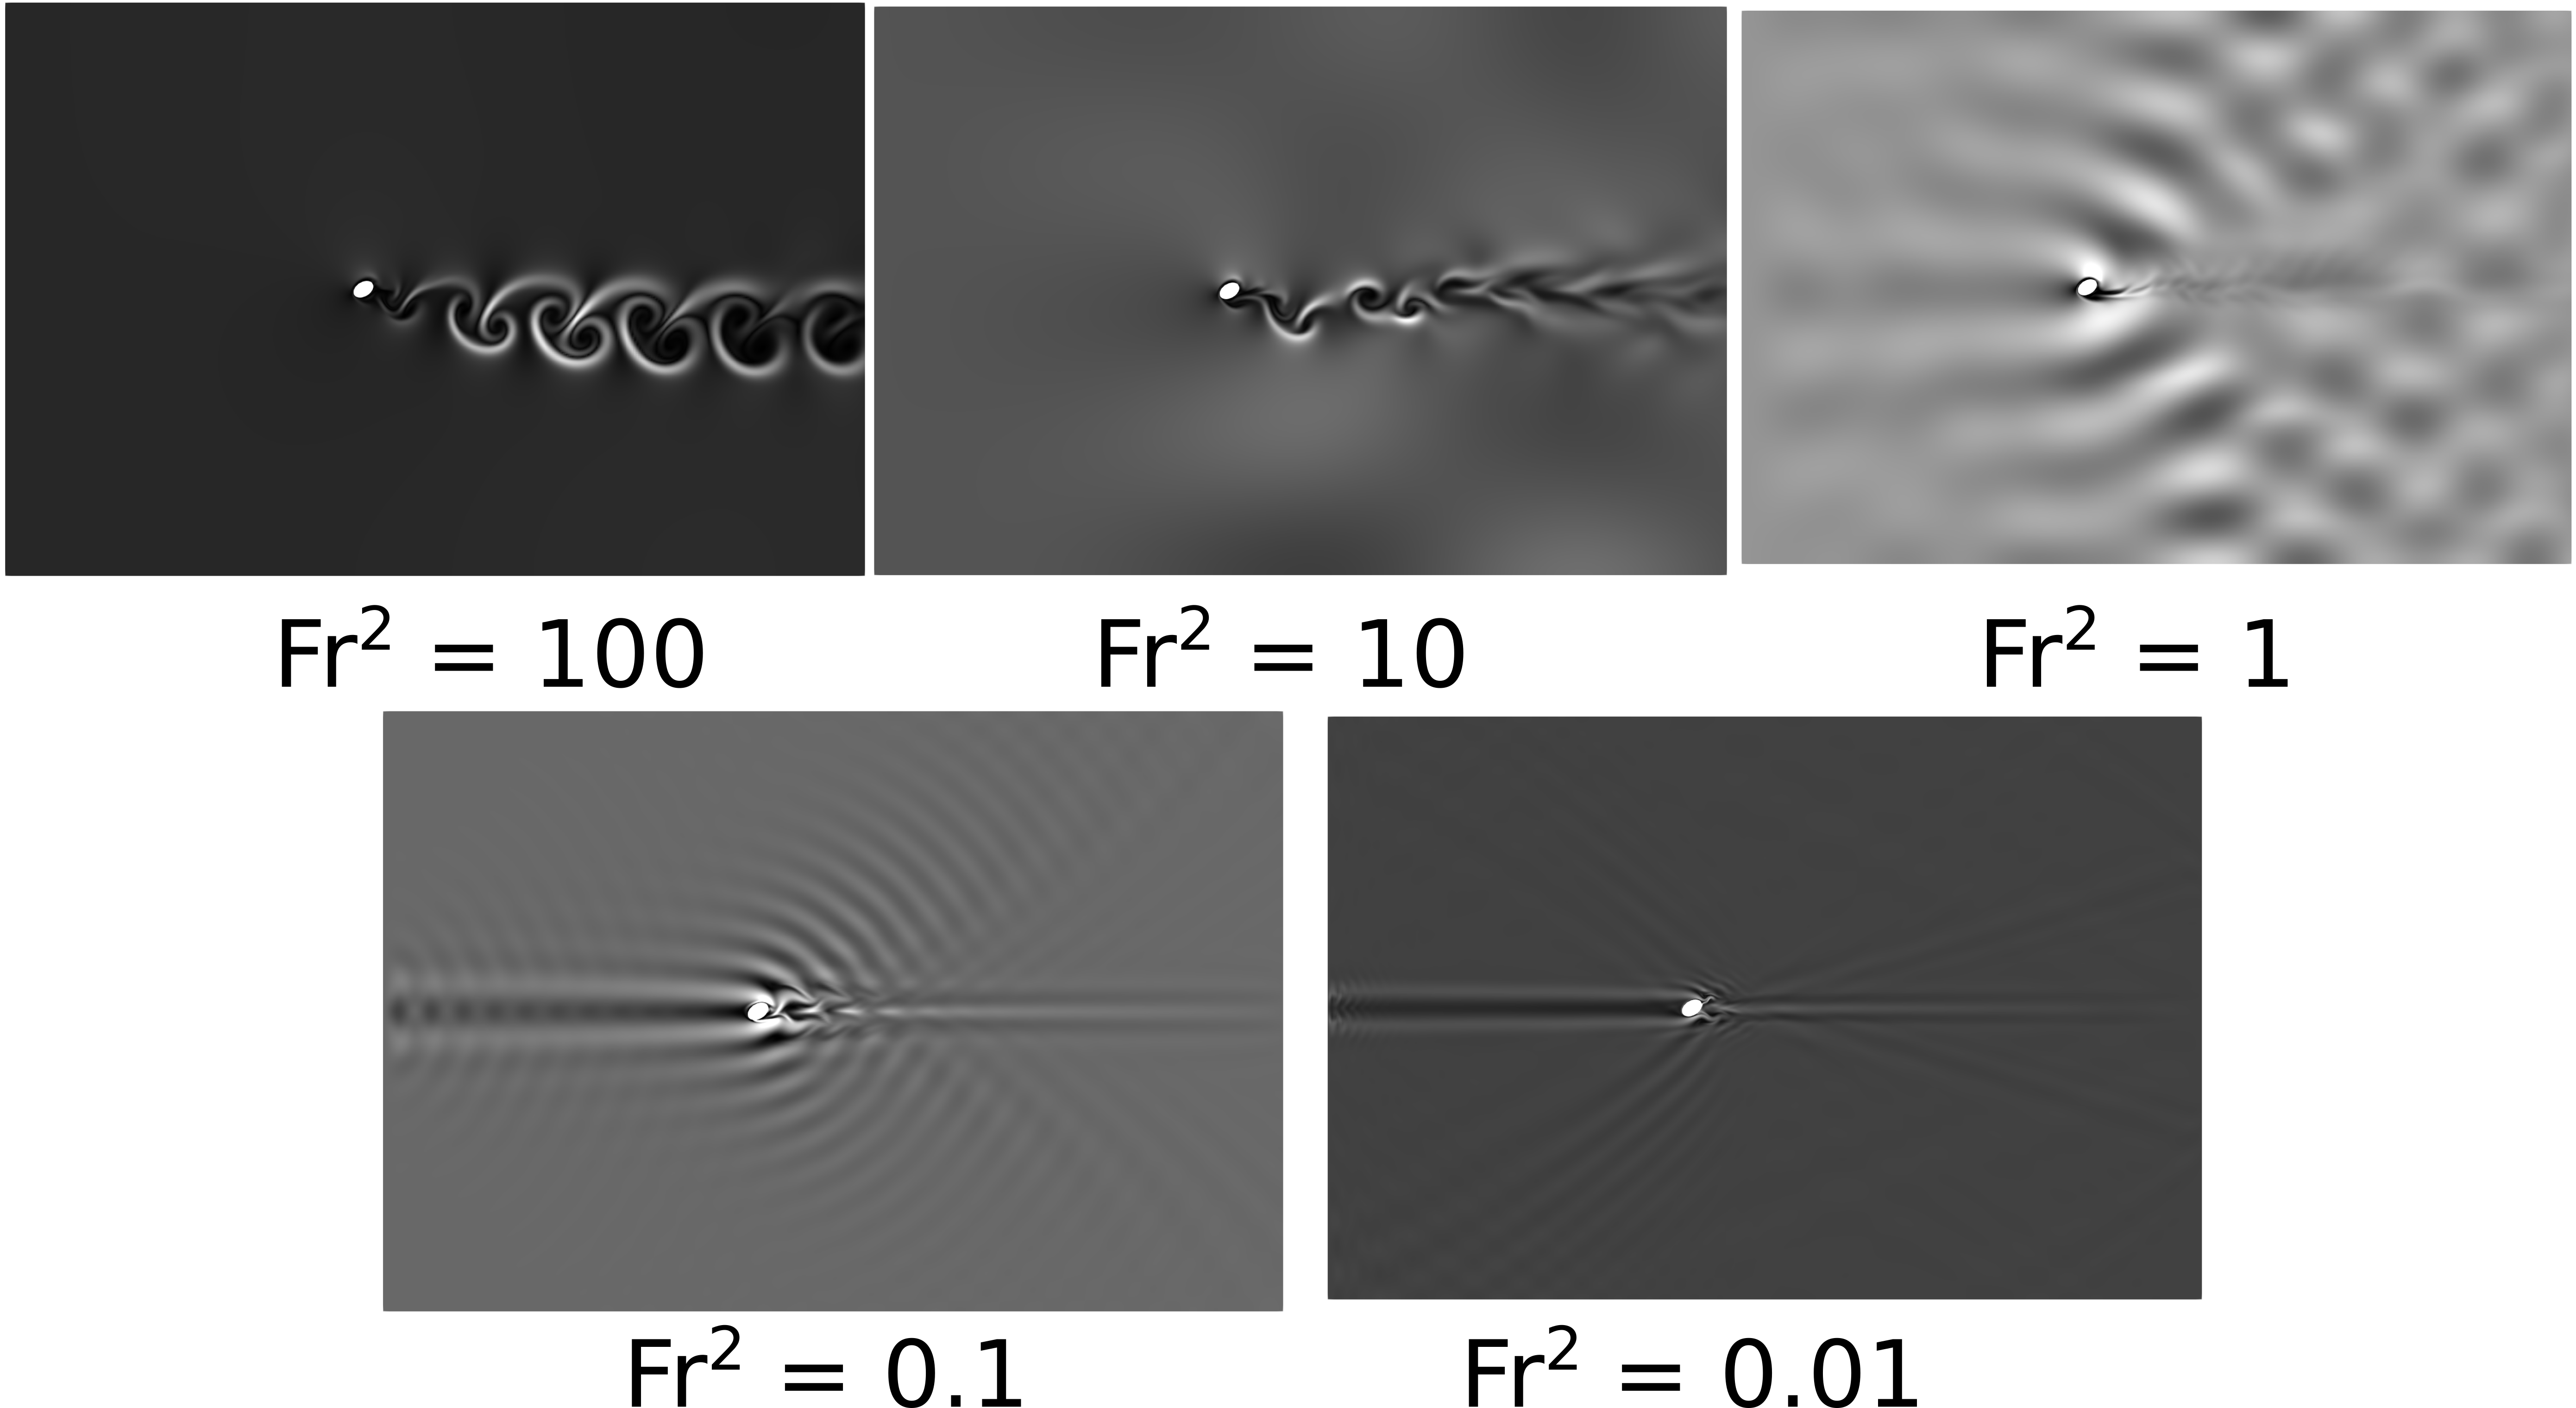
\includegraphics[width=.8\textwidth]{figures/schlierenar1p5.png}
%           \caption*{$AR = 1.5$ Schlieren}
        \end{figure}
    \end{columns}
\end{frame}

%------------------------------------------------

\begin{frame}{Cycle-averaged Drag and Lift}
    \begin{columns}[c]
        \column{.5\textwidth}
        \begin{figure}
            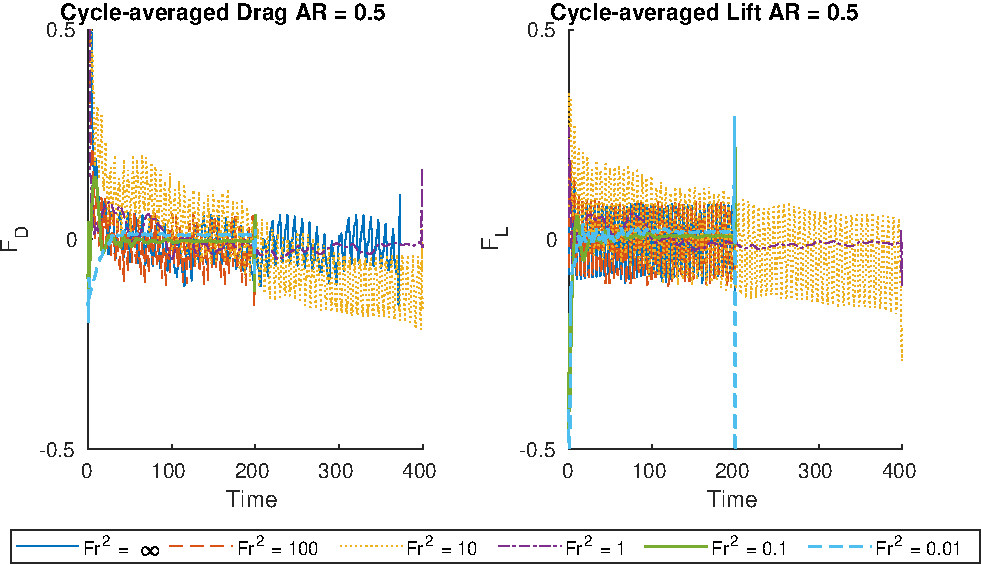
\includegraphics[width=.8\textwidth]{figures/mvmean0p5.pdf}
        \end{figure}
        \begin{figure}
            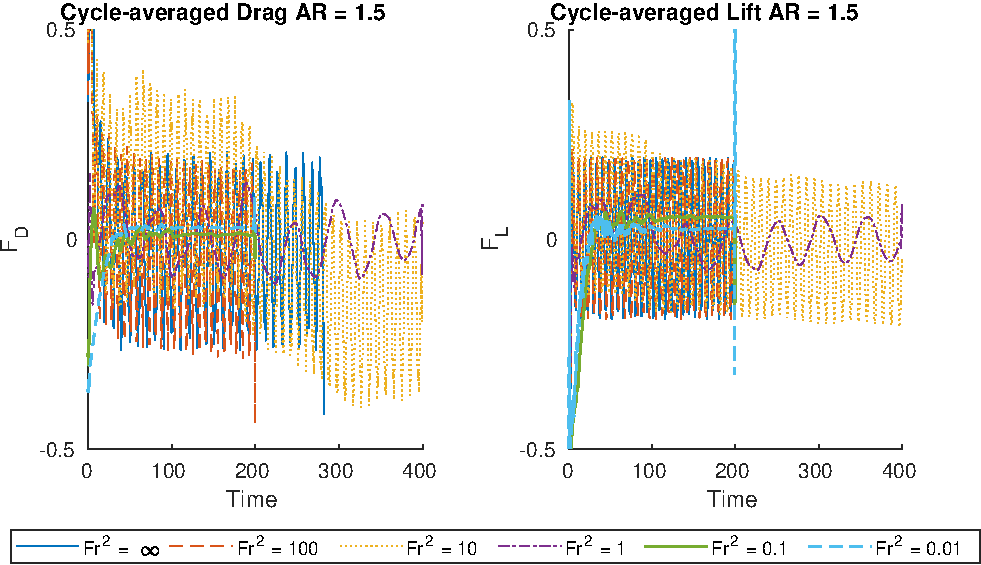
\includegraphics[width=.8\textwidth]{figures/mvmean1p5.pdf}
        \end{figure}
        \column{.5\textwidth}
        \begin{figure}
            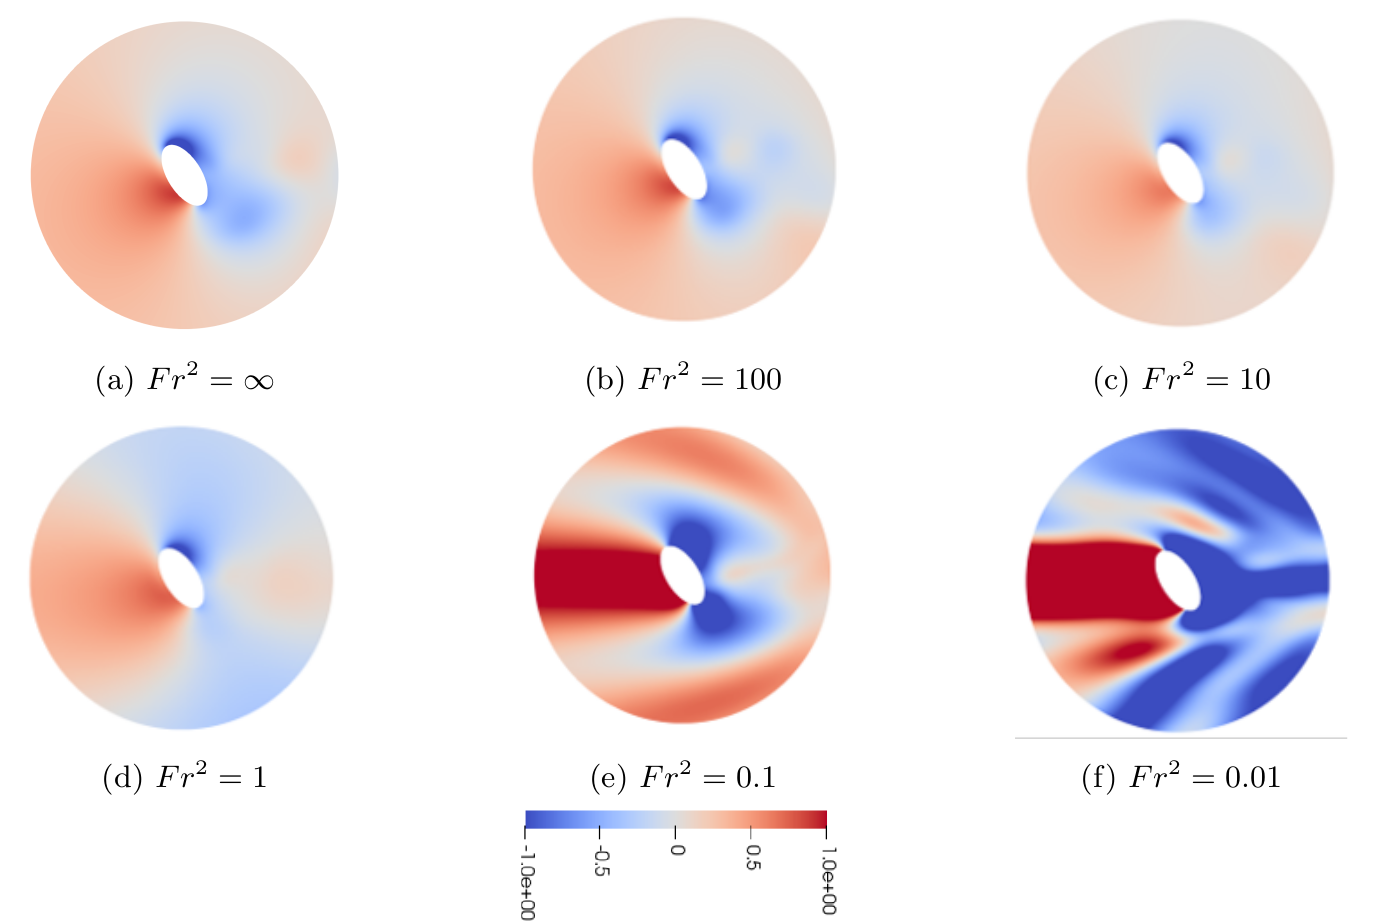
\includegraphics[width=.6\textwidth]{figures/pres_0p5.png}
        \end{figure}
        \begin{figure}
            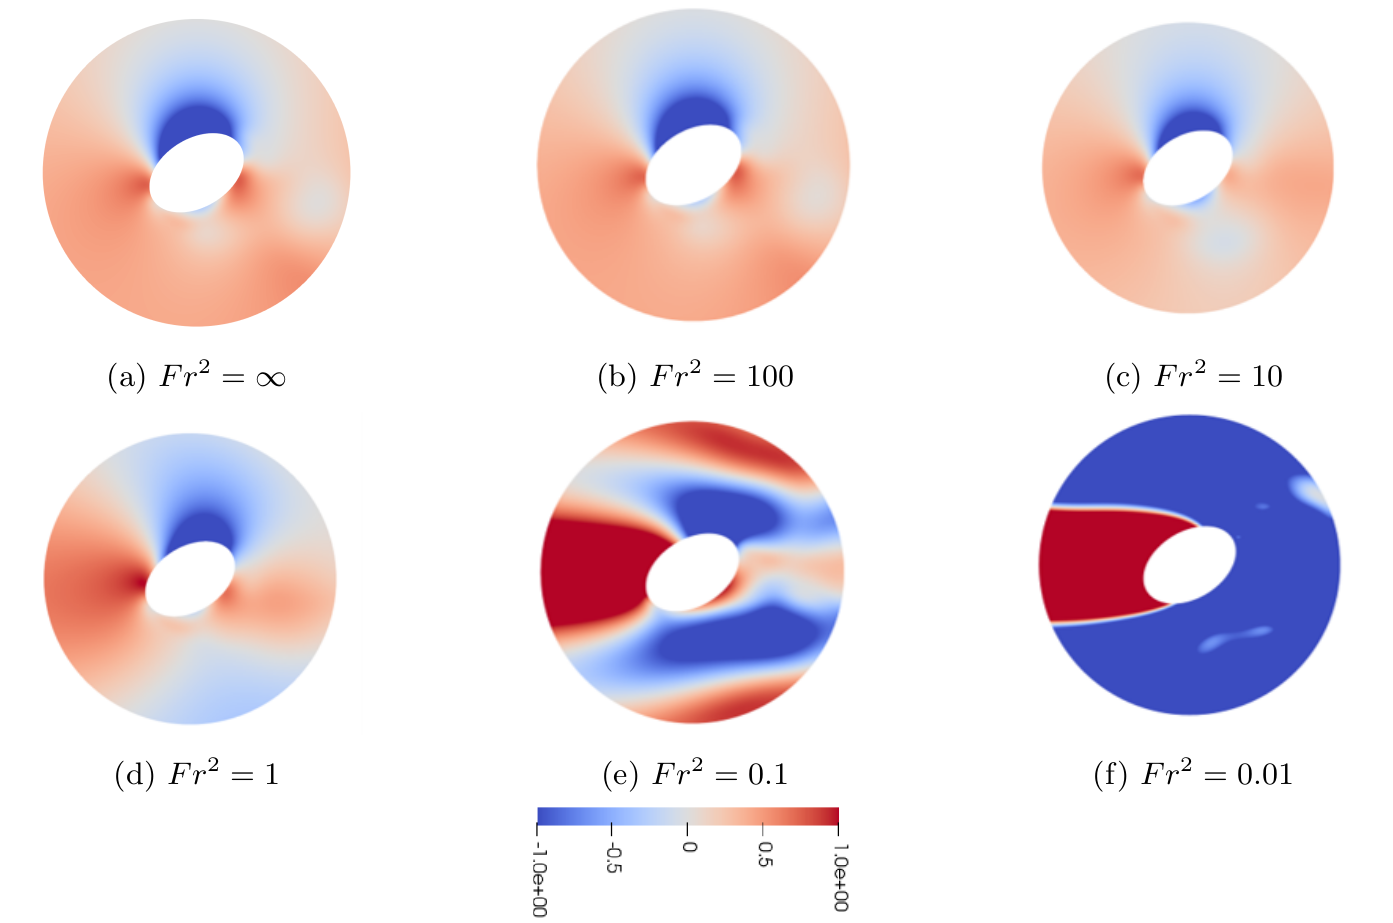
\includegraphics[width=.6\textwidth]{figures/pres_1p5.png}
        \end{figure}
    \end{columns}
\end{frame}

%------------------------------------------------

\begin{frame}{Deeper Analysis}
    \begin{itemize}
        \item Applying Hilbert transform to extract analtyic signal using FFT
        \item Follow the procedure outlined by \cite{mercier2008reflection}
        \item $\mathfrak{H}(|\nabla \rho|) = \mathfrak{F}^{-1}(2H(\mathfrak{F}(| \nabla \rho |)))$
        \item $Fr^2 = 0.1, AR = 1.5$ case
    \end{itemize}
    
    \begin{figure}
        \begin{subfigure}[b]{.45\textwidth}
            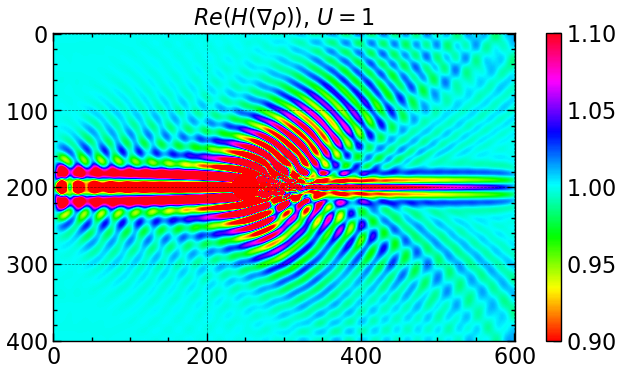
\includegraphics[width=\textwidth]{figures/ReH.png}
        \end{subfigure}
        \begin{subfigure}[b]{.45\textwidth}
            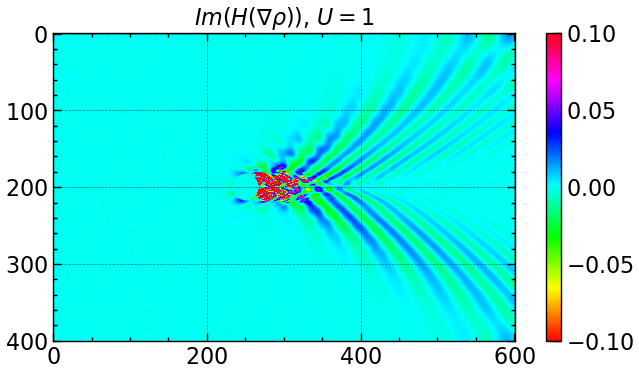
\includegraphics[width=\textwidth]{figures/ImH.png}
        \end{subfigure}
    \end{figure}
\end{frame}

%------------------------------------------------

\begin{frame}
    \Large 
    Acknowledgements\\
    \vspace{5pt}
    \normalsize
    The support and resources from the Center for High Performance Computing at the University of Utah are gratefully acknowledged.\\
    \vspace{5pt}
    \Large
    References
    \normalsize
    \bibliographystyle{jfm}
    \bibliography{ref}
\end{frame}

%----------------------------------------------------------------------------------------

\end{document}